%\documentclass[conference, oribibl]{IEEEtran}
\documentclass[runningheads,a4paper,oribibl]{llncs}
%\usepackage{llncsdoc}

% *** MISC UTILITY PACKAGES ***
%
\usepackage{amssymb}
\usepackage{verbatim}
\setcounter{tocdepth}{3}
\usepackage{adjustbox,lipsum}

\usepackage{graphicx}
\graphicspath{ {Figs/} }

\usepackage{amsmath}
\usepackage{multirow}
%\usepackage{slashbox}
\usepackage{amsfonts}

\usepackage{algpseudocode}
\usepackage{algorithm}
\usepackage{epstopdf}
\usepackage{array}
\usepackage{enumerate}

\usepackage{epstopdf}

\usepackage{url}
\usepackage{subcaption}
\captionsetup{compatibility=false}
%\urldef{\mailsa}\path|{khanhtv, mizuhito}@jaist.ac.jp|    

%ieee requirements
%\usepackage[utf8]{inputenc}
%\usepackage[T1]{fontenc}
%\usepackage{microtype} 
%\usepackage{balance}

%user definitions
\newcommand{\Nat}{{\mathbb N}}
\newcommand{\Real}{{\mathbb R}}
\newcommand{\Rat}{{\mathbb Q}}
\newcommand{\suppress}[1]{} % Comment out text.
\newcommand{\mizuhito}[1]{\{{\bf Mizuhito:~\sf #1}\}} % Highlight text.
\newcommand{\khanh}[1]{\{{\bf Khanh:~\sf #1}\}} % Highlight text.

\newcommand{\smallHead}[1]{%
    \par\vspace{.35cm}\noindent\textbf{#1}%
    \par\noindent\ignorespaces%
}

\newcommand\TTTT{%
 \textsf{T\kern-0.2em\raisebox{-0.3em}T\kern-0.2emT\kern-0.2em\raisebox{-0.3em}2}%
}

% correct bad hyphenation here
\hyphenation{op-tical net-works semi-conduc-tor}


\begin{document}
%
% paper title
% can use linebreaks \\ within to get better formatting as desired
% Do not put math or special symbols in the title.
\title{{\bf raSAT}: SMT Solver for Polynomial Constraints over Reals}

\author{Vu Xuan Tung\inst{1}, To Van Khanh\inst{2}, and Mizuhito Ogawa\inst{1}} 
\institute{
Japan Advanced Institute of Science and Technology\\
\email{\{tungvx,mizuhito\}@jaist.ac.jp}
\and 
University of Engineering and Technology, Vietnam National 
University, Hanoi \\
\email{khanhtv@vnu.edu.vn}
}

%\tableofcontents

% make the title area
\maketitle

% As a general rule, do not put math, special symbols or citations
% in the abstract
\begin{abstract}
This paper presents an SMT (Satisfiability Modulo Theory) solver {\bf raSAT} for polynomial inequality. 
It consists of a simple iterative approximation refinement, called {\bf raSAT} loop, 
which is an extension of the standard ICP (Interval Constraint Propagation) with Testing. 
Two approximation schemes consist of Interval Arithmetic (IA) and 
Testing, to accelerate SAT detection. 
If both fails, input intervals are refined by decomposition. 

ICP is robust for large degrees, but the number of boxes (products of intervals) to explore 
exponentially explodes with respect to the number of variables. 
We design strategies for boosting SAT detection on the choice of a variable to decompose
and a box to explore. 

Several heuristic measures, called {\em SAT likelihood}, {\em sensitivity}, and the number of 
unsolved atomic polynomial constraints, are compared on Zankl, Meti-tarski and Keymaera benchmarks from 
QF\_NRA category of SMT-LIB. They are also evaluated by comparing {\bf Z3 4.3}, \textbf{dReal-2.15.01} and {\bf iSAT3}. 
raSAT loop is extended with the use of the Intermediate Value Theorem to solve equality. This extension is evaluated on equalities of Zankl, Meti-tarski and Keymaera families.
We also show a simple modification to handle mixed integers, and experiments on 
AProVE benchmark from QF\_NIA category of SMT-LIB. 
\end{abstract}
% no keywords
%\keywords{Interval Arithmetic, affine arithmetic, SMT, polynomial constraints, 
%Testing, abstract DPLL.}


% For peer review papers, you can put extra information on the cover
% page as needed:
% \ifCLASSOPTIONpeerreview
% \begin{center} \bfseries EDICS Category: 3-BBND \end{center}
% \fi
%
% For peerreview papers, this IEEEtran command inserts a page break and
% creates the second title. It will be ignored for other modes.
% \IEEEpeerreviewmaketitle

\section{Introduction}
{\em Polynomial constraint solving} over reals (resp. integers) is to find an instance from reals
(resp. integers) that satisfies given polynomial inequality/equality. 
%For instance, $\exists x y. -y^2 + (x^2 - 1) y - 1 > 0 \wedge -x^2 - y^2 + 4 > 0$ is 
%such an example. This is an easy formula, but proving its satisfiability and 
%showing a satisfiable instance (e.g., $x = 1.8$, $y=0.9$) are not so easy.  
%its satisfiability and a satisfiable instance 
%(e.g., $x = 1.8$, $y=0.9$) are not so easy.  		
%
Many applications are reduced to solving polynomial constraints, e.g.,
\begin{itemize}
\item {\bf Locating roundoff and overflow errors}, 
which is our motivation~\cite{Ngoc:2009:ORE:1685167.1685421}. 
%DSP decoders in practice are defined by reference algorithms in C using floating point arithmetic. 
%In embedded systems, often it is replaced with fixed point arithmetic, 
%which may cause visible noises. 
%and locating such roundoff error source is not easy. 
%For instance, consider DSP decoder like mpeg4. Usually, the decoder definition is given by a reference 
%algorithm in C, which uses floating point number. 
%In an embedded system, it is tempting to replace floating 
%point into fixed point numbers. However, naive replacement would cause 

\item {\bf Automatic termination proving}, 
which looks for a suitable ordering~\cite{Lucas:2008:CCS:1361735.1361760}, 
e.g., \TTTT\footnote{\url{http://cl-informatik.uibk.ac.at/software/ttt2/}}, 
AProVE\footnote{\url{http://aprove.informatik.rwth-aachen.de}}. 
%as a solution of polynomial constraints. 

\item {\bf Loop invariant generation}. 
e.g., both~\cite{Colon} with Farkas's lemma, %and is reduced to degree $2$ polynomials. 
and~\cite{Sankaranarayanan:2004:NLI:982962.964028} are reduced to non-linear constraint solving.
%matrix multiplications. 
%degree $2$ polynomial constraints. 
%Farkas's lemma uses products of matrices, and it requires solving polynomial constraints of degree 2.

\item {\bf Hybrid system}. SMT solvers are often backend engines~\cite{Sankaranarayanan04constructinginvariants}. 
%\item {\bf Mechanical contrnol design}. 
%Proportional-integral-derivative controllers are simple but widely used, and designing parameters is 
%reduced to polynomial constraints~\cite{control}. 
%Fujitsu used polynomial constraints solving to design PID control of HDD head movement
\end{itemize}	

Solving polynomial constraints on reals is decidable~\cite{tarski}, 
though that on integers is undecidable ({\em Hilbert's 10th problem}). 
Quantifier elimination by cylindrical algebraic decomposition (QE-CAD)~\cite{qecad} 
is a well known technique, and 
implemented in Mathematica, Maple/SynRac, Reduce/Redlog, QEPCAD-B, and recently 
in some SMT solvers~\cite{Jovanovic13,smtrat}.   % Refer Z3 4.3 = nlast and SMT-RAT
QE-CAD solves more than the satisfiability, and is DEXPTIME. % and hardly works up to 8 variables and degree 10.
By restricting on the satisfiability, {\em Variant quantifier elimination}~\cite{Hong2012883} reduces to 
polynomial optimization problems, which are solved by Groebner basis in EXPTIME. 

A practical alternative is Interval Constraint Propagation({\em ICP})\cite{benhamou:hal-00480814}, 
%which are used in SMT solver community, 
which is implemented in {\bf iSAT3}~\cite{isat}, {\bf dReal}~\cite{dRealCADE13}, and \textbf{RSolver}~\cite{rsolver}. 
ICP is based on an over-approximation by Interval Arithmetic, and iteratively refines by
interval decompositions. 
Although ICP is often not complete for UNSAT detection with unbounded intervals, 
it is practically often more efficient than algebraic computation. 
%%%%%%%%%%%%%
\begin{comment}
For polynomial inequality 
$\exists x_1 \in (a_1,b_1) \cdots x_n \in (a_n,b_n) . \wedge_{i} f_i > 0$, 
\begin{itemize}
\item If $\exists x_1 \in (a_1,b_1) \cdots x_n \in (a_n,b_n) . \wedge_{i} f_i > 0$ is SAT, 
ICP eventually detects it. 
\item If $\exists x_1 \in [a_1,b_1] \cdots x_n \in [a_n,b_n] . \wedge_{i} f_i \geq 0$ is UNSAT, 
ICP eventually detects it
\end{itemize}
under the assumptions of bounded intervals. 
\begin{figure}[ht]
%\begin{minipage}[b]{1.0\linewidth}
\centering
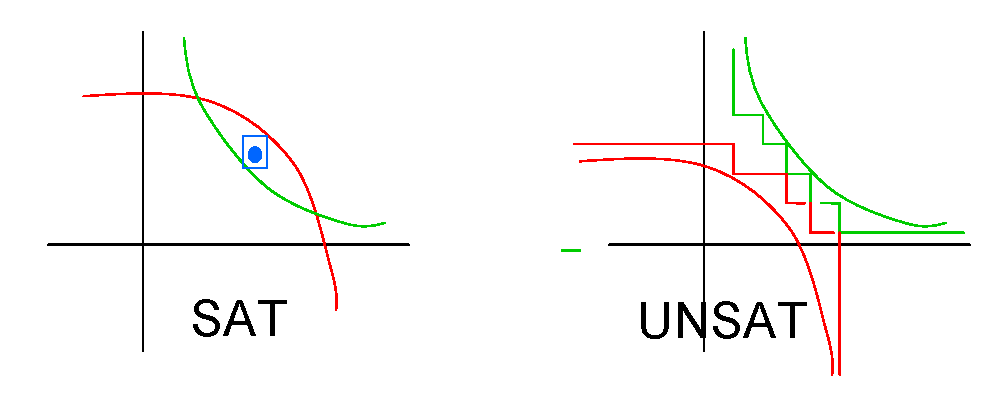
\includegraphics[height=1.2in,width=3.4in]{FigCompleteness.eps} 
\caption{SAT and UNSAT detection by ICP} 
\label{fig:complete} 
%\end{minipage}
\end{figure} 

The boundary part is reduced to polynomial equality checking, 
which would be solved by using algebraic methods, like Groebner basis. 
Alternatively, by loosening equality to $\delta$-equality, 
$\delta$-completeness is obtained~\cite{dRealCADE13}. 
\end{comment}
%%%%%%%%%%%%%

This paper presents an SMT solver {\bf raSAT} for polynomial constraints over reals. 
It consists of a simple iterative approximation refinement, called {\bf raSAT} {\em loop}, 
which adds Testing to boost SAT detection to a standard ICP. 
Two approximation schemes consist of Interval Arithmetic (over-approximation) and 
Testing (under-approximation), to boost SAT detection. 
If both the estimation by a Interval Arithmetic and Testing fail, input intervals are refined by decompositions. 
%
The features of {\bf raSAT} are, 
\begin{itemize}
\item {\bf raSAT} loop, which adds Testing to boost SAT detection to a standard ICP, 
\item various Interval Arithmetics support, e.g., 
Affine intervals~\cite{Messine_extensionsof,Ngoc:2009:ORE:1685167.1685421,VanKhanh201227}, 
\item sound use of floating point arithmetic, i.e., 
outward rounding in Interval Arithmetic~\cite{Hickey:2001:IAP:502102.502106}, 
%round up/down for the upper/lower bounds in Interval Arithmetic, 
and confirmation of an SAT instance by an error-bound guaranteed floating point package {\bf iRRAM}\footnote{% 
\tt http://irram.uni-trier.de}. 
\end{itemize}
%This design is more on SAT detection oriented, since from our preliminary experiences, 
%if the target problems have several hundred variables, solvable cases in practice are 
%either SAT or UNSAT with small UNSAT core. 
%Thus, acceleration of SAT detection and finding UNSAT core will be keys for scalability. 
%As \textbf{iSAT3}, \textbf{raSAT} applies outward rounding~\cite{Hickey:2001:IAP:502102.502106} 
%in Interval Arithmetic to avoid soundless bugs due to round-off error of floating arithmetic operations. 
%As a consequence, answers of raSAT (SAT or UNSAT) (SAT instances found in Testing is verified by 
%\textbf{iRRAM}) are guaranteed to be sound.

ICP and {\bf raSAT} loop are robust for large degrees, but the number of boxes (products of intervals) 
grows exponentially. 
First, we target on polynomial inequalities, and design SAT detection-directed strategies on 
the choice of a variable to decompose, a box to explore, and a variable to generate multiple test cases. 
They are based on heuristic measures, {\em SAT likelihood}, {\em sensitivity}, and the number of 
unsolved atomic polynomial constraints. 
The combinations are examined on Zankl, Meti-tarski and Keymaera benchmarks from 
QF\_NRA of SMT-LIB, to find clear differences from random choices. 
We also show two extensions, (1) handling polynomial equality by using the Intermediate Value Theorem, 
and (2) polynomial constraints over integers (e.g., AProVE benchmark in QF\_NIA). 
These results are also compared with {\bf Z3 4.3}, \textbf{dReal-2.15.01} and {\bf iSAT3}. 

%%%%%%%%%%%
\suppress{
ICP is robust for larger degrees, but the number of boxes (products of intervals) to explore 
exponentially explodes when variables increase. 
Thus, design of strategies for selecting variables to decompose and boxes to explore is crucial 
for efficiency. Our strategy design is, 
\begin{itemize}
\item a box with more possibility to be SAT is selected to explore, which is estimated by 
several heuristic measures, called {\em SAT likelihood}, 
and the number of unsolved atomic polynomial constraints, and
\item a more influential variable is selected for multiple test cases and decomposition, 
which is estimated by {\em sensitivity}. 
\end{itemize} 
%Note that {\em SAT likelihood} and {\em sensitivity} are estimated using Interval Arithmetic. 
%Especially, the latter can be applied only with Affine intervals. 
}
%%%%%%%%%%%
{\bf raSAT} also applies incremental search not to fall into local optimals. 
\begin{itemize}
\item {\bf Incremental widening}. 
Starting {\bf raSAT} loop with a smaller initial interval, and if it is UNSAT, enlarge the input intervals
and restart. 
\item {\bf Incremental deepening}. 
Starting with the bound that each interval will be decomposed no smaller than it. 
If neither SAT nor UNSAT is detected, set a smaller bound and restart. 
\end{itemize} 
%Efficient UNSAT core % with error bound guaranteed floating point arithmetic 
%is left for future work. 

%%%%%%%%%%%%
\begin{comment}
They are compared on Zankl, Meti-Tarski and Keymaera benchmarks from 
QF\_NRA category of SMT-LIB\footnote{\tt http://www.smtlib.org/}. 
They are also evaluated by comparing 
{\bf Z3~4.3}\footnote{\tt http://z3.codeplex.com}, {\bf iSAT3} and \textbf{dReal-2.15.01}. 
Another advantage of {\bf raSAT} is the ease to handle mixed integers, 
and experiments on AProVE benchmark from QF\_NIA category of SMT-LIB compares {\bf raSAT} with 
{\bf Z3 4.3}. 
Although {\bf Z3 4.3} performs the best, {\bf raSAT} shows comparable SAT detection on 
very large problems (e.g., with several hundred variables) with the combination of 
{\em SAT likelihood} and {\em sensitivity}. 
\end{comment}
%%%%%%%%%%%%


\section{ICP overview and \textbf{raSAT} loop}
\label{sec:raSATloop} 

\sloppy

Our target problems is a nonlinear constraint, especially over real numbers. 
That over integer numbers will be briefly shown in Section~\ref{sec:NIA}.
We mainly discuss on polynomial inequalities, and later in Section~\ref{sec:eq},
we show an extension to cover polynomial equality based on the
Intermediate Value Theorem. 

\begin{definition}
A polynomial inequality constraint is
\[\varphi: \exists x_1 \in I_1 \cdots x_n \in I_n. \bigwedge
\limits_{j=1}^m \psi_j(x_1,\cdots,x_n)\]
where $\psi_j(x_1,\cdots,x_n)$ is an atomic polynomial inequality (API) of
the form $p_j(x_1,...,x_n) > 0$ with $p_j(x_1,...,x_n)$ is a polynomial.
We denote the set of variables appearing in $p_j$ by $var(p_j)$. 
\end{definition}

Note that $\varphi$ is equivalent to 
${\exists x_1 \ldots x_n. (\bigwedge \limits_{i=1}^n x_i \in I_i) \wedge
  (\bigwedge \limits_{j=1}^m \psi_j(x_1,\cdots,x_n))}$. 
We call ${\bigwedge \limits_i x_i \in I_i}$ an {\em interval constraint}, and 
we refer $\bigwedge \limits_{j=1}^m \psi_j(x_1,\cdots,x_n)$ by
$\psi(x_1,\cdots,x_n)$.
We denote the set of solutions of the constraint $\psi(x_1,\cdots, x_n)$ as
${\mathbb{S}(\psi(x_1,\cdots, x_n)) = \{(r_1,\cdots, r_n) \in \Real^n \mid
  \psi(r_1. \cdots, r_n) \text{ holds}\}}$.

We first review Interval Constraint Propagation (ICP)\cite{benhamou:hal-00480814}, and then introduce
\textbf{raSAT} (refinement of approximations for SAT) loop~\cite{VanKhanh201227}.
The main difference is that {\bf raSAT} loop has Testing after the estimation
by Interval Arithmetic (IA) to boost SAT detection.
Note that both ICP and {\bf raSAT} are suffered from roundoff errors of
the floating arithmetic. To guarantee the soundness, IA adopts
outward rounding~\cite{Hickey:2001:IAP:502102.502106} for the estimation of lower/upper bounds of intervals.
In {\bf raSAT}, when Testing says SAT, it is confirmed with
the error bound guaranteed package {\bf iRRAM}. 

\begin{comment}
\begin{figure}[ht]
\begin{minipage}[b]{1.0\linewidth}
\centering
\begin{tabular}{c@{\qquad}c}
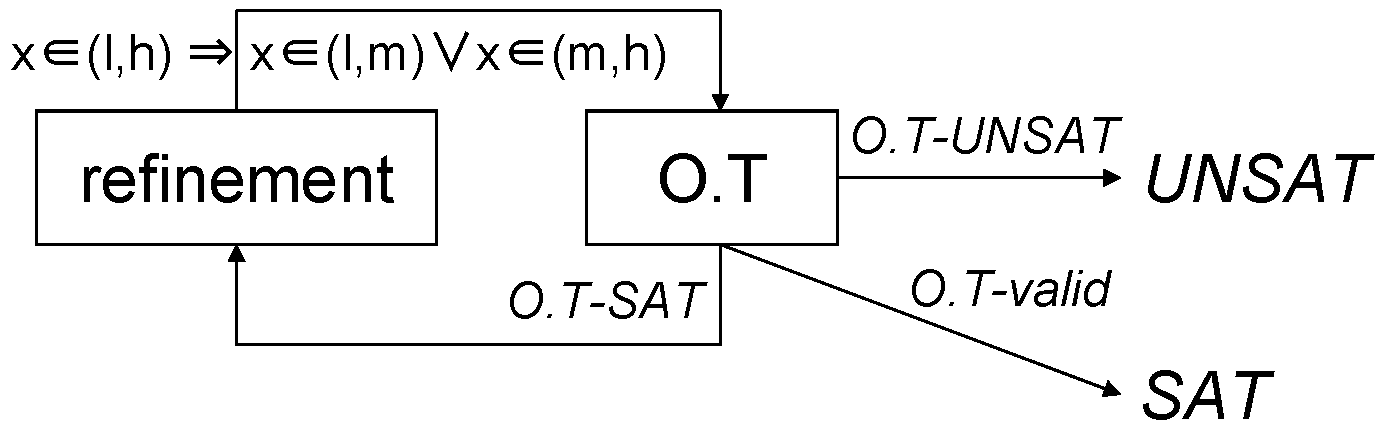
\includegraphics[height=0.6in,width=1.7in]{OTloop.png} & 
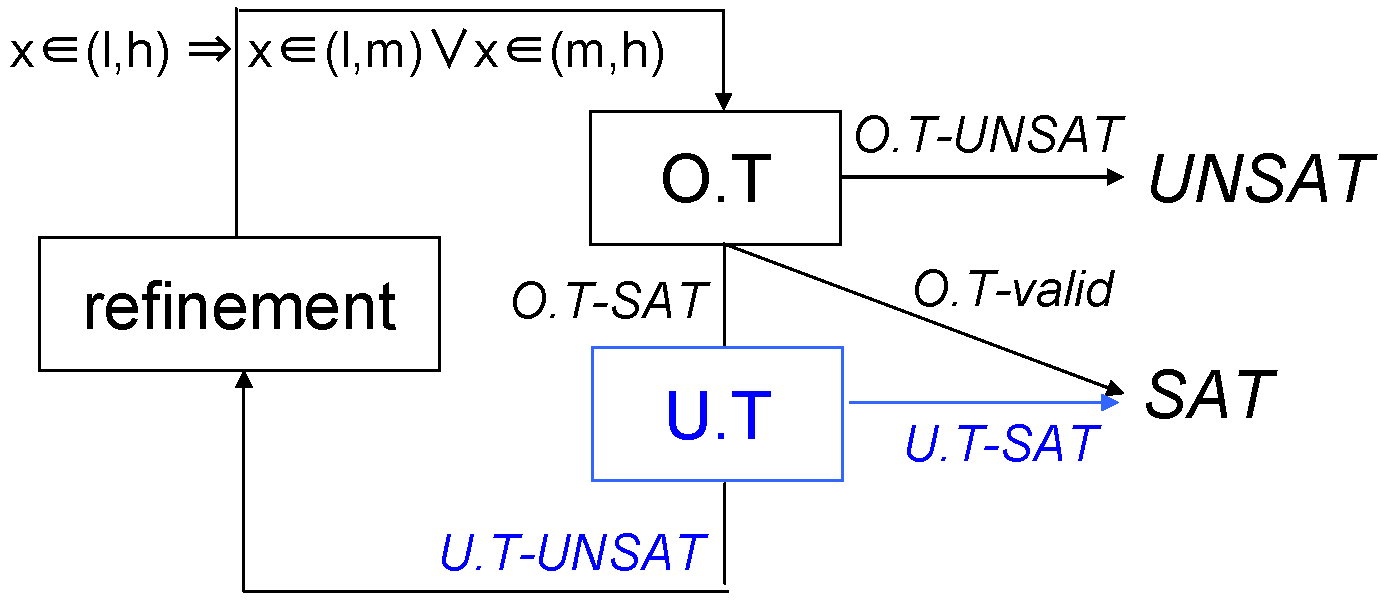
\includegraphics[height=0.9in,width=1.7in]{rasatloop.png} \\   
\mbox{(a) ICP loop} & \mbox{{\bf raSAT} loop} \\
\end{tabular}
\end{minipage} 
\caption{Refinement loops} 
\label{fig:OTrefine} 
\end{figure}
\end{comment}

\subsection{ICP overview}
\sloppy 
%\exists x_1 \ldots x_n. (\underbrace{\bigwedge \limits_i x_i \in I_i}_{I}) \wedge 
%                       (\underbrace{\bigwedge \limits_j \psi_j(x_1,\cdots,x_n)}_{P})
%and $\circ \in \{>, <, \geq, \leq\}$.
%%%%%%%%%%%
\begin{comment}
  Initially, interval constraints have a form of the conjunction
  $\bigwedge \limits_i x_i \in I_i$, and later by refinement,
  $x_i \in I_i$ is decomposed into a clause $\bigvee_k x_i \in I_{i_k}$, which makes a CNF. 

\begin{example} \label{examp:poly_ieq}
$\exists x \in (-1,3)~y \in (2,4) . (x^3y - y^4 > 0) \wedge (y^3 -xy >0)$
is an example of a polynomial inequality with 2 variables and 2 APIs. 

If, for instance, $x \in (-1,3)$ and $y \in (2,4)$ are refined to smaller intervals
such that 
${\exists x \in (-1,1) y \in (2,4) . (x^3y - y^4 > 0) \wedge (y^3 -xy >0)} \vee 
 {\exists x \in (1,3) y \in (2,4) . (x^3y - y^4 > 0) \wedge (y^3 -xy >0)}$, 
it results a CNF 
${(x \in (-1,1) \vee x \in (1,3)) \wedge (y \in (2,4)) \wedge (x^3y - y^4 > 0)
  \wedge (y^3 -xy >0)}$.
%(only the CNF formula $(x \in (-1,1) \vee x \in (1,3)) \wedge (y \in (2,4))$
%is given to SAT solver).
%\mizuhito{could you fulfill? Direct encoding seems a DNF?}. 
\end{example}

As an SMT (SAT modulo theory) problem, 
boolean variables are assigned to each $x_i \in I_{i_k}$, 
and truth assignments is produced by a SAT solver, 
which are proved or disproved by a background theory $T$
whether it satisfies $\psi(x_1,\cdots,x_n)$. 

\sloppy
As notational convention, $m$ (the lower case) denotes 
an assignment ${\{x_i \mapsto r_i \mid i \in \{1, \cdots, n\}\}}$ from real numbers $r_i$'s to $x_i$'s, and 
$M$ (the upper case) denotes a truth assignment on $x_i \in I_{i_k}$'s. 
We write $m \in M$ when for all $i \in \{1, \cdots, n\}$, we have $c_i \in I_{i_k}$ for all $x_i \in I_{i_k}$'s that are assigned true by $M$. 

We assume {\em very lazy theory learning}~\cite{dpll}, and 
a backend theory $T$ is applied only for a full truth assignment $M$. 
\end{comment}
%%%%%%%%%%%

%We regard $M$ as a conjunction $\bigwedge \limits_i x_i \in I_{i_j}$. 
%%%%%%%%%%%
\begin{comment}
\begin{itemize}
\item If an instance $m$ satisfies $\psi(x_1,\cdots,x_n)$, we denote $m \models_T \psi(x_1,\cdots,x_n)$. 
\item If each instance $m$ with $m \in M$ satisfies $\psi(x_1,\cdots,x_n)$, 
we denote $M \models_T \psi(x_1,\cdots,x_n)$. 
\end{itemize}
%%%%%%%%%%%

\begin{definition} \label{def:app}
Let $F = \exists x_1 \in I_1 \cdots x_n \in I_n. \psi(x_1,\cdots,x_n)$. 
For a truth assignment on $M$, $F$ is 
\begin{itemize}
\item $T$-valid if $M \models_T \psi(x_1,\cdots,$ $x_n)$, 
\item $T$-satisfiable ($T$-SAT) if $m \models_T \psi(x_1,\cdots,x_n)$ 
for some $m \in M$, and 
\item $T$-unsatisfiable ($T$-UNSAT) if $M \models_T \neg \psi(x_1,\cdots,x_n)$. 
\end{itemize}
If $T$ is clear from the context, we simply say valid, satisfiable, and unsatisfiable. 
\end{definition}

%%%%%%%%%%%%%
\suppress{
Then, Fig. \ref{fig:T_result} illustrates Definition~\ref{def:app}. 
\begin{figure} [ht]
\centering
\begin{minipage}[b]{0.45\linewidth}
  \includegraphics[height=1.8in,width=1.9in]{T_result.eps}
\caption{Results of a target constraint $F$ in a theory $T$}
\label{fig:T_result}
\end{minipage}
\quad
\begin{minipage}[b]{0.45\linewidth}
   \includegraphics[height=2.2in,width=2.3in]{frame_app.eps}
\caption{{\bf raSAT} loop}
\label{fig:frame}
\end{minipage}
\end{figure}
}
%%%%%%%%%%%%%%%%%%%%%%%%%%%%%%%%

\begin{definition} \label{def:ApproxTheory}
Let $T, O.T, U.T$ be theories. 
\begin{itemize}
\item $O.T$ is an {\em over-approximation theory} (of $T$) 
if $O.T$-UNSAT implies $T$-UNSAT, and
\item $U.T$ is an {\em under-approximation theory} (of $T$)
if $U.T$-SAT implies $T$-SAT. 
\end{itemize}
It is easy to see that $O.T$-valid implies $T$-valid. 
\end{definition}
\end{comment}

%Note that $O.T$-valid can be regarded as $U.T$, since $O.T$-valid implies $T$-valid, thus $T$-SAT. 
%ICP applies Interval Arithmetic (as an over approximation) during the checking of background theory. 
%Later in Section~\ref{sec:approximation}, we will instantiate Interval Arithmetic as $O.T$. 
%Adding to this, {\bf raSAT} introduces Testing (as an under-approximation) to accelerate SAT detection. 

%\subsection{Over-Approximation Theory Refinement}
%\label{sec:soundness}

%From now on, we focus on a \emph{polynomial inequality} such that 
%$I_i$ and $\psi_j(x_1,\cdots,x_n)$ are an open interval $(a_i,b_i)$ and 
%an atomic polynomial inequaltiy (API) $f_j > 0$, respectively. 

%%%%%%%%%%%%%%%%%%%%%%%%% Actual start of the section 

Algorithm~\ref{Al:ICP} describe the basic ICP for solving polynomial inequalities.
Let $\psi = \bigwedge\limits_{j=1}^mg_j(x_1, \cdots, x_n) > 0$ be a target constraint. 
\begin{algorithm}
\begin{algorithmic}[1]
\State $S \gets \{B_0\}$ \Comment Set of boxes
\While {$S \neq \emptyset$}
  \State $B \gets S.choose()$ \Comment Get one box from the set
  \State $B' \gets prune(B, \psi)$
  \If {$B' = \emptyset$} \Comment The box does not satisfy the constraint
  	\State $S \gets S \setminus \{B\}$
  	\State continue
  \ElsIf {$B'$ satisfies $\psi$ by using \emph{IA}}
  	\State \Return SAT
  \Else \Comment \emph{IA} cannot conclude the constraint $\implies$ \emph{Refinement} Step
  	\State $\{B_1, B_2\} \gets split(B')$ \Comment split $B'$ into two smaller boxes $B_1$ and $B_2$	
  	\State $S \gets (S \setminus \{B\}) \cup \{B_1, B_2\}$
  \EndIf
\EndWhile
\State \Return UNSAT
\end{algorithmic}
\caption{ICP starting from the initial box $B_0 = I_1 \times \cdots \times I_n$}
\label{Al:ICP}
\end{algorithm}

\noindent
where two functions $prune(B,\psi)$ and $split(B)$ satisfy 
\begin{itemize}
\item If $B' = prune (B, \psi)$,
  then $B' \subseteq B $ and $ B' \cap \mathbb{S}(\psi) = B \cap \mathbb{S}(\psi)$. 
\item If $\{B_1, B_2\} = split (B)$,
  then $B = B_1 \cup B_2$ and $B_1 \cap B_2 = \emptyset$. 
\end{itemize}

Since ICP concludes SAT (line 8) only when it finds a box in which the constraint
becomes valid by IA. It is also suffered from roundoff errors, and 
the basic ICP cannot conclude the satisfiability of equations. 
In contrast, although the number of boxes increase exponentially,
ICP always detects SAT of an inequality constraint 
$\exists x_1 \in (a_1,b_1) \cdots x_n \in (a_n,b_n) . \wedge_{j} g_j > 0$
if the $split$ is fairly applied and each $I_j$ is bounded. 
However, ICP may miss to detect UNSAT.
Limitations for detecting UNSAT come from the \emph{kissing} and \emph{convergent} cases
in Fig.~\ref{fig:limit}.  The left shows a kissing case 
$x^2 + y^2 < 2^2 \wedge (x-4)^2 + (y-3)^2 < 3^2$ such that 
$\overline{\mathbb{S}(- x^2 - y^2 + 2^2 > 0)} \cap
 \overline{\mathbb{S}(- (x-4)^2 - (y-3)^2 + 3^2 > 0)} = \{(x,y) \mid (1.6, 1.2)\}$. 
Thus, it cannot be separated by the covering by (enough small) boxes. 
%Thus, there are no coverings to separate them. 
%$x^2 + y^2 < 2^2$ and $(x-4)^2 + (y-3)^2 < 3^2$. 
The right shows a convergent case 
$y > x + \frac{1}{x} \wedge y < x \wedge x > 0$,
i.e., $xy > x^2 + x \wedge y < x \wedge x > 0$.
The latter does not appear if all intervals $I_j$ are finitely bounded. 
%The open box is $(0,\infty) \times (0,\infty)$ and 
%There are no finite coverings to separate them. 
%$y > x + \frac{1}{x}$ and $y < x$ for $x > 0$. 
\begin{figure}[ht]
%\begin{minipage}[b]{1.0\linewidth}
\centering
\begin{tabular}{cc}
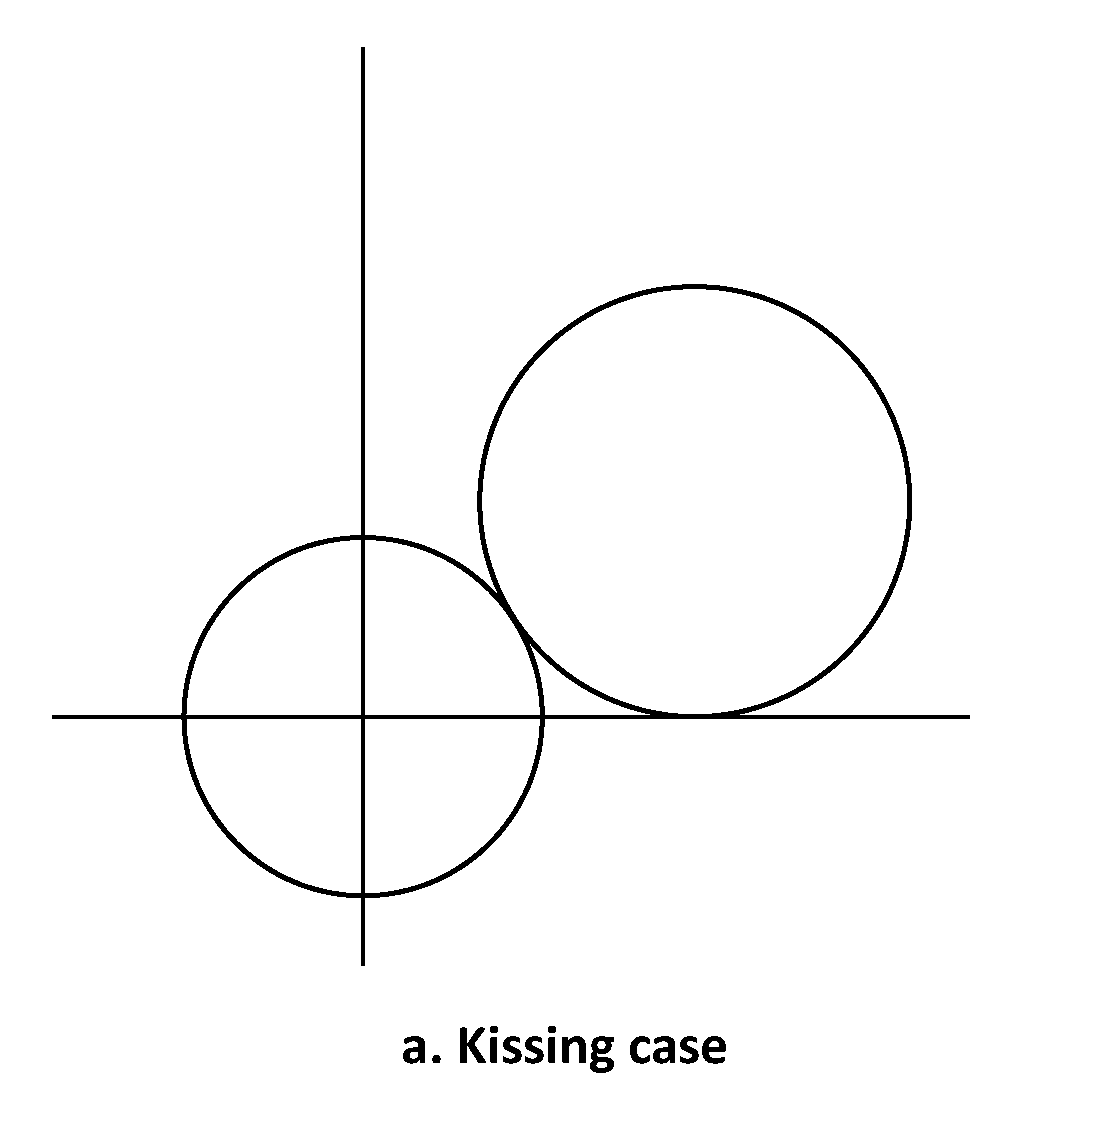
\includegraphics[height=1in,width=1.05in]{kissing.eps} &
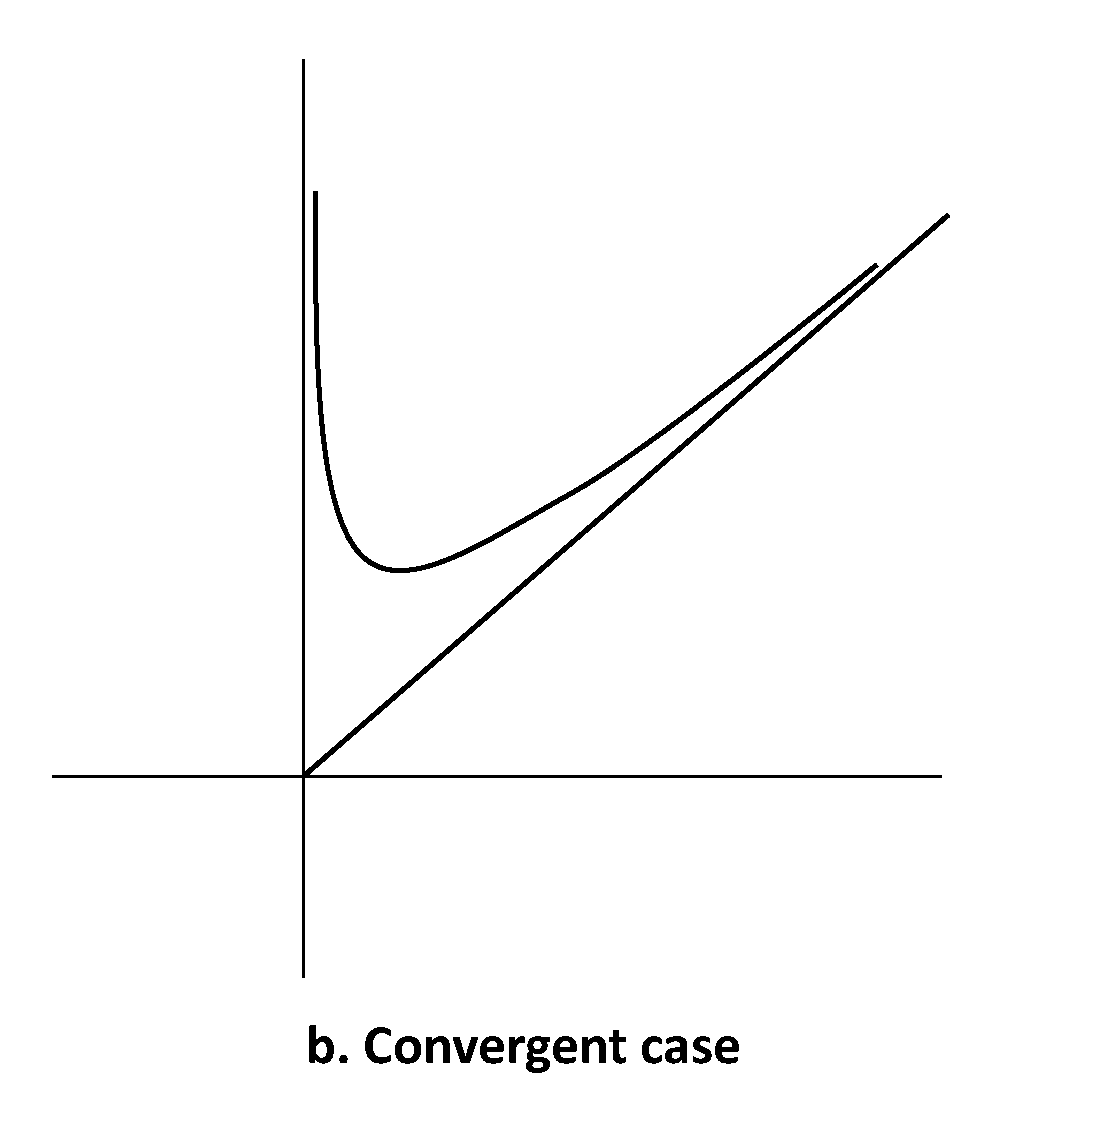
\includegraphics[height=1in,width=1.05in]{convergence.eps}
\end{tabular}
\caption{Limitations for detection of UNSAT} 
\label{fig:limit} 
%\end{minipage}
\end{figure} 


%%%%%%%%%%
\suppress{
\begin{itemize}
\item if $\exists x_1 \in (a_1,b_1) \cdots x_n \in (a_n,b_n) . \wedge_{j} g_j > 0$ is SAT, 
ICP eventually detects it, and 
\item if $\exists x_1 \in [a_1,b_1] \cdots x_n \in [a_n,b_n] . \wedge_{j} g_j \geq 0$ is UNSAT, 
ICP eventually detects it, 
\end{itemize}
under the assumptions of fair decomposition and bounded intervals $(a_i,b_i)$ for all $i \in \{1, \cdots, n\}$. 
We will prepare terminology and briefly review this fact. 
}
%%%%%%%%%%%%
\suppress{
\begin{definition} \label{def:poly}
A polynomial inequality is a bounded quantification 
$\exists x_1 \in I_1 \cdots x_n \in I_n. \psi(x_1,\cdots,x_n)$ 
such that 
\begin{itemize}
\item each $I_i$ is an open interval $x_i \in (a_i,b_i)$, and 
\item $\psi(x_1,\cdots,x_n)$ is a conjunction of $f_j > 0$ 
where $f_j$ is a polynomial over $\{x_1, \cdots, x_n\}$. 
\end{itemize}
$f_i > 0$ is called an atomic polynomial inequality (API). 
We denote $\mathbb{S}(F) = \{x \in \Real^n \mid F ~\text{holds}\}$.
\end{definition}

\begin{example} \label{examp:poly_ieq}
$\exists x \in (-1,3)~y \in (2,4) . (x^3y - y^4 > 0) \wedge (y^3 -xy >0)$
is an example of a polynomial inequality with 2 variables and 2 APIs. 
\end{example}
}
%%%%%%%%%%%%%%%%%%%%%%

%%%%%%%%%%%%%%
\begin{comment}
\begin{definition}
An \emph{open box} of dimension $n$ is a set $(a_1,b_1) \times \cdots \times (a_n,b_n)$ 
where $a_i, b_i \in \Real, a_i \leq b_i$.  
For $\mathfrak{a} = (a_1, \cdots, a_n)$ and $\mathfrak{b} = (b_1, \cdots, b_n)$, 
we denote $(a_1,b_1) \times \cdots \times (a_n,b_n)$ by $(\mathfrak{a}, \mathfrak{b})$. 
\end{definition}

The set of all open boxes is a basis of Euclidean topology on $\Real^n$. 
In $\Real^n$, a set $U$ is compact if, and only if, $U$ is a bounded closed set. 
We denote a closure of a set $U$ by $\overline{U}$. 
%
Since a polynomial is continuous, 
$\mathbb{S}(\bigwedge \limits_{j=1}^m g_j > 0)$ is an open set. 
Note that $\Rat$ is dense in $\Real$, and an SAT instance in reals can be replaced with one in rationals. 

%%%%%%%%%%%%%%%%%%%%%%%%%%%%%%
\suppress{
\begin{lemma} \label{cor:rattoreal}
For a polynomial inequality
$F = \exists x_1 \in I_1 \cdots x_n \in I_n. \bigwedge \limits_{j=1}^m f_j > 0$, 
If there exists an SAT instance of F in $\Real^n$, there exists also in $\Rat^n$. 
\end{lemma}

\begin{lemma} \label{cor:refinement}
Suppose that $a_j < b_j$ for $1 \leq j \leq n$ and $f_i$'s are polynomials. 
Assume $a_k < c < b_k$ for some $k$. 
Then, 
$\exists x_1 \in (a_1,b_1) \cdots x_n \in (a_n,b_n). \bigwedge \limits_{i=1}^m f_i > 0$ 
is SAT (resp. UNSAT) if, and only if, 
$\exists x_1 \in (a_1,b_1) \cdots x_k \in (a_k,c) \cdots x_n \in (a_n,b_n). 
 \bigwedge \limits_{i=1}^m f_i > 0 
 \vee 
 \exists x_1 \in (a_1,b_1) \cdots x_k \in (c,b_k) \cdots x_n \in (a_n,b_n)). 
 \bigwedge \limits_{i=1}^m f_i > 0$ 
is SAT (resp. UNSAT). 
\end{lemma}

\begin{pf}
We show for the SAT case. If-part is obvious. For only-if-part, 
since $\mathbb{S}(\bigwedge \limits_{i=1}^m f_i > 0)$ is an open set, 
if $y \in (a_1,b_1) \times \cdots \{c\} \cdots \times (a_n,b_n)$ satisfies 
$\bigwedge \limits_{i=1}^m f_i > 0$, 
there exists $x_1 \in (a_1,b_1) \cdots x_k \in (a_k,c) \cdots x_n \in (a_n,b_n)$
(also $x_1 \in (a_1,b_1) \cdots x_k \in (c,b_k) \cdots x_n \in (a_n,b_n)$) that satisfies
$\bigwedge \limits_{i=1}^m f_i > 0$. 
\end{pf}

Lemma~\ref{cor:rattoreal} says that proving SAT of $F$ in $\Real$ is reduced to 
that in $\Rat$. 
Lemma~\ref{cor:refinement} says that, in the refinement step, we can apply refinement 
$x_k \in (a_k,b_k)$ to $x_k \in (a_k,c) \vee x_k \in (c,b_k)$, 
instead of $x_k \in (a_k,c] \vee x_k \in (c,b_k) $
(i.e., $c$ is ignored). 
}
%%%%%%%%%%%%%%%%%%%%%%%%%%%%%%

%Initially, interval constraints consists of conjunction only. Later, by refinements,
%it becomes a CNF. 

Note that an Interval Arithmetic used in ICP is a converging theory. 

\begin{definition} \label{def:completeOT}
Let
$\varphi = \exists x_1 \in I_1 \cdots x_n \in I_n. \bigwedge \limits_{j=1}^m g_j > 0$
be a polynomial inequality such that each $I_i$ is bounded. 
An theory $T$ is {\em converging} 
if, for each $\delta > 0$ and $c = (c_1, \cdots, c_n) \in I_1 \times \cdots \times I_n$, 
there exists $\gamma > 0$ such that $T$ can concludes that  
for all $x_i \in (c_i - \gamma, c_i + \gamma)$, $i=1,\cdots, n$, we have 
 $\bigwedge \limits_{j=1}^m (g_j(c) - \delta < g_j(x) < g_j(c) + \delta)$. 
\end{definition}

%$O.T$ refinement loop is shown in Fig.~\ref{fig:OTrefine}~(a). 
%A standard ICP based algorithm of an SMT solver applies it with
%$O.T$ as a classical interval arithemtic. 
%The variation of interval arithemtic will be presented in Section~\ref{sec:approximation}. 

\begin{definition} 
Let
$\varphi = \exists x_1 \in I_1 \cdots x_n \in I_n. \bigwedge \limits_{j=1}^m g_j > 0$
for $I_i = (a_i,b_i)$.
A refinement strategy is {\em fair}, if, for each $c_i \in (a_i,b_i)$ and $\gamma > 0$, 
a decomposition of $I_i$ for each $i$ eventually occurs in $(c_i - \gamma, c_i + \gamma)$ 
(as long as neither SAT nor UNSAT is detected). 
\end{definition}

\begin{theorem} \label{th:RelComp}
Let
$\varphi = \exists x_1 \in I_1 \cdots x_n \in I_n. \bigwedge \limits_{j=1}^m g_j > 0$
for $I_i = (a_i,b_i)$.
Assume that
each $(a_i,b_i)$ is bounded, and a refinement strategy is fair. 
Then, 
\begin{itemize}
\item if $\exists x_1 \in (a_1,b_1) \cdots x_n \in (a_n,b_n) . \wedge_{j} g_j > 0$ is SAT, 
ICP eventually detects it, and
\item if $\exists x_1 \in [a_1,b_1] \cdots x_n \in [a_n,b_n] . \wedge_{j} g_j \geq 0$ is UNSAT, 
ICP eventually detects it.  
\end{itemize}
\end{theorem}


\begin{proof} 
The former is proved by the fact that, if $\varphi$ is SAT, there exists a non-empty neighborhood (open box) 
in $\cap~\mathbb{S}(g_j > 0)$. 
If the box decomposition strategy is fair, the refinement will eventually find such an open box. 

For the latter, assume that 
$\overline{\varphi} = \exists x_1 \in [a_1,b_1] \cdots x_n \in [a_n,b_n] . \wedge_{j} g_j \geq 0$ is UNSAT. 
Thus, $\cap~\overline{\mathbb{S}(g_j > 0)} = \emptyset$. 
Let $\delta_{j,k} = min \{|g_j(\bar{x}) - g_k(\bar{x})| \mid \bar{x} \in I_1 \times \cdots \times I_n\}$. 
Since $g_j$'s are continuous and $\overline{I_i}$'s are compact, $\delta_{j,k}$ is well defined,
and $\delta_{j.k} > 0$ for some $j,k$. 
Let $\delta = \frac{min \{ \delta_{j,k} \}}{2}$. 
Since IA is converging, there exists $\gamma > 0$ for $\delta > 0$ 
satisfying Definition~\ref{def:completeOT}, and fair decomposition eventually finds open boxes
such that $\mathbb{S}(g_j \ge 0)$ and $\mathbb{S}(g_k \ge 0)$ are separated. 
\qed
\end{proof}
\end{comment}
%%%%%%%%%%%%%%


\subsection{raSAT loop}

We extend ICP with Testing to accelerate SAT detection, which is called {\bf raSAT}
loop~\cite{VanKhanh201227}.  %Fig.~\ref{fig:OTrefine}~(b). 
Algorithm~\ref{Al:raSATLoop} displays {\bf raSAT} loop where $\psi = \bigwedge\limits_{j=1}^mg_j(x_1, \cdots, x_n) > 0$ is the target constraint. 
\begin{comment}
\begin{enumerate}
\item When an Interval Arithmetic detects UNSAT (resp. valid), conclude UNSAT (resp. SAT). 
\item When an Testing detects SAT, conclude SAT. 
\item If neither holds, a refinement is applied. 
\end{enumerate}
\end{comment} 

\begin{algorithm}
\begin{algorithmic}[1]
\While {$\Pi$ is satisfiable} \Comment Some more boxes exist
\State $\pi = \{x_i \in I_{ik} \mid i \in \{1,\cdots, n\}, k \in \{1,\cdots, i_k\} \} \gets $
a solution of $\Pi$ 	
\State $B \gets $ the box represented by
$\bigwedge\limits_{i=1}^n\bigwedge\limits_{k=1}^{i_k}x_i \in I_{ik}$

\If {$B$ does not satisfy $\psi$ by using \emph{IA}}
\State $\Pi \gets \Pi \wedge \neg(\bigwedge\limits_{i=1}^n\bigwedge\limits_{k=1}^{i_k}x_i \in I_{ik})$
  \ElsIf {$B$ satisfies $\psi$ by using \emph{IA}}
\State \Return SAT
  \ElsIf {$B$ satisfies $\psi$ by using \emph{Testing}} \Comment Different from ICP
\State \Return SAT
\Else \Comment Neither \emph{IA} nor \emph{Testing} conclude the constraint $\implies$
\emph{Refinement} Step
\State choose $(x_i \in I_{ik}) \in \pi$ such that $\forall k_1 \in \{1,\cdots, i_k\} I_{ik} \subseteq I_{ik_1}$
\State $\{I_1, I_2\} \gets split(I_{ik})$ \Comment split $I_{ik}$
into two smaller intervals $I_1$ and $I_2$
\State $\Pi \gets \Pi \wedge (x_i \in I_{ik} \leftrightarrow (x_i \in I_1 \vee x_i \in I_2))
\wedge \neg(x_i \in I_1 \wedge x_i \in I_2)$

\EndIf
\EndWhile
\State \Return UNSAT
\end{algorithmic}
\caption{\textbf{raSAT} loop starting from the initial box
  $\Pi = \bigwedge\limits_{i=1}^n x_i \in I_i^0$}
\label{Al:raSATLoop}
\end{algorithm}

Our design of an SMT solver {\bf raSAT} adapts various Interval Arithmetic,
and applies two main heuristics (the use of Affine Intervals enable us to apply the latter).
\begin{itemize}
\item Incremental widening intervals, and incremental deeping search 
(Section~\ref{sec:incsearch}). 
\item 
Heurstic measures {\em SAT-likelihood} and {\em sensitivity}, 
for selection of a variable to decompose (line 11 of Algorithm~\ref{Al:raSATLoop}) and
a box to explore (line 13, Algorithm~\ref{Al:raSATLoop}). (Section~\ref{sec:SATheuristics}). 
\end{itemize} 

%{\bf raSAT} prepares various Interval Arithmetics. %as $O.T$ as in following, 
%whereas currently only random tesing (\emph{k-random ticks}, 
%which consists of periodical $k$-test instances with a random offset) is prepared as $U.T$. 


\subsection{Interval Arithmetic} \label{sec:approximation}

%%%%%%%%%%%%
\suppress{A typical theory for $O.T$ and $U.T$ are an Interval Arithmetic and Testing, respectively. 
We say {\em IA-valid}, {\em IA-SAT}, and {\em IA-UNSAT}, when it is $O.T$-valid, $O.T$-SAT, and 
$O.T$-UNSAT, respectively. 
Similarly, we say {\em test-SAT} when it is $U.T$-SAT and {\em test-UNSAT} when $U.T$-UNSAT. 
Note that either IA-valid or test-SAT implies SAT, and IA-UNSAT implies UNSAT, 
whereas IA-SAT and test-UNSAT can conclude neither.} 

%We instantiate Testing to $U.T$ in Section~\ref{sec:raSATloop}. 
\suppress{
\begin{definition}\label{def:Testing}
%For $\exists x_1 \in (a_1,b_1) \cdots x_n \in (a_n,b_n). \bigwedge \limits_{i=1}^m f_i(x_1,\cdots,x_n) > 0$, 
Let $M = \bigwedge \limits_{i=1}^m x_i \in (a_i,b_i)$ and 
${\mathcal P} = \bigwedge \limits_{i=1}^m f_i(x_1,\cdots,x_n) > 0$. 
%
Let a choice function $\theta : (\Real \times \Real)^n \rightarrow \Real^n$ 
such that $\theta(M) \in (a_1,b_1) \times \cdots \times (a_n,b_n)$. 
Testing is a finite set $\Theta$ of choice functions. Then, we say 
\begin{itemize}
\item ${\mathcal P}$ is \emph{Test-SAT} under $M$ if $\theta(M)$ holds ${\mathcal P}$ 
for some $\theta \in \Theta$, and 
\item ${\mathcal P}$ is \emph{Test-UNSAT} under $M$ if $\theta(M)$ never holds ${\mathcal P}$ 
for each $\theta \in \Theta$. 
\end{itemize} 
%We denote $I \models_{test(\theta)} P$ if $\bigwedge \limits_{i=1}^m f_i(\theta(I)) > 0$ holds.
\end{definition}
}
%%%%%%%%%%%%%%%%


{\bf raSAT} prepares various Affine Intervals~\cite{Comba93affinearithmetic},
adding to Classical Interval (CI)~\cite{moore}. 
%which keep lower and upper bounds.
Although precision of the estimations is incomparable, 
Affine Intervals preserve a part of the dependency among values, which are lost in CI. 
For instance, $x - x$ is evaluated to $(-2,2)$ for $x \in (2,4)$ by CI, but $0$ by an Affine Interval.

Affine Interval introduces \emph{noise symbols} $\epsilon$, 
which are interpreted as values in $(-1,1)$. 
For instance, $x = 3 + \epsilon$ describes $x \in (2,4)$, and 
$x - x = (3 + \epsilon) - (3 + \epsilon)$ is evaluated to $0$. 
The drawback is that the multiplication without dependency might be less precise than CI.
Affine Intervals also cannot represent infinite intervals, e.g., $(0,\infty)$, 
since it becomes $\infty + \infty~\epsilon$. 
Forms of Affine Intervals vary by choices how to approximate multiplications. They are,
\begin{enumerate}[(i)]
\item $\epsilon \epsilon'$ is replaced with a fresh noise symbol 
($AF$)~\cite{Comba93affinearithmetic}, 
\item $\epsilon \epsilon'$ is reduced to the fixed error noise symbol 
$\epsilon_{\pm}$ ($AF_1$ and $AF_2$) \cite{Messine_extensionsof},
\item $\epsilon \epsilon'$ is replaced with $(-1,1) \epsilon$ 
(or $(-1,1) \epsilon'$) ($EAI$)~\cite{Ngoc:2009:ORE:1685167.1685421},
\item $\epsilon \epsilon$ is reduced to fixed noise symbols 
$\epsilon_+$ or $\epsilon_{-}$ ($AF_2$) \cite{Messine_extensionsof}, 
\item Chebyshev approximation of $x^2$ introduces a noise symbol $|\epsilon|$ 
as an absolute value of $\epsilon$ with 
$\epsilon \epsilon = |\epsilon| |\epsilon| = |\epsilon| + (-\frac{1}{4}, 0)$ and
$\epsilon |\epsilon| = \epsilon + (-\frac{1}{4}, \frac{1}{4})$ \cite{VanKhanh201227}. 
%(Fig.~\ref{fig:chevabs}). 
%\item keeping products of noise symbols up to degree $2$ ($\epsilon_i \epsilon_j$),
\end{enumerate} 

%%%%%%%%%%%%%%%%%
\suppress{
\begin{remark}
For Affine Intervals, \emph{sensitivity}~\cite{ngocsefm} of a variable
is a possible range of the absolute value of the coefficient of its corresponding $\epsilon$. 

%In Example~\ref{examp:sensitivity}, $CAI$ estimates the coefficient of $|\epsilon_1|$ as $\textbf{3}$, 
%which has the largest sensitivity and indicates $x$ the most influencial. 

Note that Affine Interval works only for bounded intervals. 
For instance, $\infty + \infty \epsilon$ represents $(-\infty,\infty)$, which says nothing. 
Narrowing intervals as an incremental search (Section~\ref{sec:incsearch})
partially depends on this fact. 
That is, if $\pm \infty$ is contained in an interval, first give finite upper/lower bounds and
search within these bounds using an Affine Interval.
If UNSAT is concluded, then enlarge to the whole intervals using CI. 
\end{remark}
}
%%%%%%%%%%%%%%%%%


\begin{example} \label{examp:sensitivity}
Let $g = x^3 - 2xy$ with $x = (0,2)$ ($x = 1 + \epsilon_1$) and $y=(1,3)$ ($y = 2+\epsilon_2$), 
we have,
\begin{itemize}
\item $AF_2$ estimates the range of $g$ as 
$-3 - \epsilon_1 - 2\epsilon_2 + 3\epsilon_+ + 3\epsilon_{\pm}$, thus $(-9,6)$,
\item $CAI$ estimates the range of $g$ as 
$(-4,-\frac{11}{4}) + (-\frac{1}{4}, 0)\epsilon_1 - 2\epsilon_2 +
 \textbf{3}|\epsilon_1| + (-2,2)\epsilon_{\pm}$, thus $(-8,4.5)$.
\end{itemize}
\end{example}


%%%%%%%%%%%%%%%%%%%%%%%%%%
\suppress{
\begin{figure}[ht]
\begin{minipage}[b]{1.0\linewidth}
\centering
\begin{tabular}{ll}
\includegraphics[height=1.6in,width=1.7in]{chev1.pdf} &
\includegraphics[height=1.6in,width=1.7in]{chev2.pdf}
\end{tabular}
\caption{Chebyshev approximation of $x^2$ and $x~|x|$}
\label{fig:chevabs}
\end{minipage}
\end{figure}

$CAI$ \cite{tapas12} consists of (ii) and (v), which keeps better precision than iv)
for multiplicatins of the same variables, e.g., Taylor expansion. 
%To improve precision in estimating upper and lower bounds of polynomials, we apply 
%\textbf{Affine Arithmetic} such as $AF_1$, $AF_2$ \cite{af}, $CAI$ ~\cite{tapas12} 
%instead of Classical Interval \cite{moore}. 
%Note that upper and lower bounds estimated by IA are over-approximation bounds of polynomials.
}
%%%%%%%%%%%%%%%%%%%%%%%%%%
\suppress{
\begin{definition}
%For $\exists x_1 \in (a_1,b_1) \cdots x_n \in (a_n,b_n). \bigwedge \limits_{i=1}^m f_i(x_1,\cdots,x_n) > 0$, 
Let $M = \bigwedge \limits_{i=1}^m x_i \in (a_i,b_i)$ and 
${\mathcal P} = \bigwedge \limits_{i=1}^m f_i(x_1,\cdots,x_n) > 0$. 
%
Let $\delta_i^l$ and $\delta_i^u$ be lower and upper bounds of $f_i(x_1,\cdots,x_n)$ 
estimated by IA for $x_i \in (a_i,b_i)$. Then, we say 
%
%\vspace*{0.5em}
\begin{itemize}
\item ${\mathcal P}$ is \emph{IA-VALID} under $M$, if IA evaluates 
$~\forall i \in [1,m].~\delta_i^l > 0$,
%\vspace*{0.33em}
\item ${\mathcal P}$ is \emph{IA-UNSAT} under $M$, 
$~\exists i \in [1,m].~\delta_i^u \leq 0$, and 
\item ${\mathcal P}$ is \emph{IA-SAT} under $M$, if 
$(\exists j \in [1,m].~\delta_j^l \leq 0)\; \wedge \; 
	(\bigwedge \limits_{i=1}^m \delta_i^u > 0)$.
\end{itemize} 
\end{definition}

IA-VALID and IA-UNSAT safely reason satisfiability (SAT) and unsatisfiability (UNSAT), 
respectively. However, IA-SAT cannot conclude SAT. 
}
%%%%%%%%%%%%%%%%%



\section{SAT directed Strategies of {\bf raSAT}} \label{sec:strategy}

ICP is affected less with the degree of polynomials, but affected most with the number of variables. 
Starting with $\varphi = \exists x_1 \in I_1 \cdots x_n \in I_n. \bigwedge \limits_{j=1}^m g_j > 0$, 
$I_1 \times \cdots \times I_n$ is decomposed into exponentially many boxes, 
and $F$ becomes the disjunction of existential formulae corresponding to these boxes.
%since the decomposition phase would lead exponentially large number of boxes will be generated.
The detection of UNSAT requires exhaustive search on all boxes, and finding a small UNSAT core
is the key. This is often observed by {\bf Z3} where UNSAT either is quickly detected or leads to timeout. 
For SAT detection, the keys will be a strategic control not to fall into local optimal and
a strategy to choose most likely decomposition/boxes. 

\subsection{Incremental search} \label{sec:incsearch}

Two incremental search strategies are prepared in {\bf raSAT}, 
(1) {\em incremental widening}, and (2) {\em incremental deepening}. 
Let
$\varphi = \exists x_1 \in I_1 \cdots x_n \in I_n. \bigwedge \limits_{j=1}^m g_j > 0$
for $I_i = (a_i,b_i)$. %where $a_i, b_i$ would be $\pm \infty$. 

\subsubsection*{Incremental widening}
Given $0 < \delta_0 < \delta_1 < \cdots$, 
{\em incremental widening} starts with 
$F_0 = \exists x_1 \in I_1 \cap (-\delta_0 , \delta_0) \cdots x_n \in I_n \cap (-\delta_0 , \delta_0). 
\bigwedge \limits_{j=1}^m g_j > 0$, 
and if it stays  UNSAT, then enlarge the intervals as 
$F_1 = \exists x_1 \in I_1 \cap (-\delta_1 , \delta_1) \cdots x_n \in I_n \cap (-\delta_1 , \delta_1). 
\bigwedge \limits_{j=1}^m g_j > 0$. This continues until either SAT, timeout, or
a given bound of repeatation (Fig.~\ref{fig:incwid} (a)). 

Note that if $\delta_i = \infty$, we cannot use an Affine Interval
For instance, $(-\infty,\infty) = \infty \epsilon$ does not make sense.
In {\bf raSAT}, $AF_2$ is used if $\delta_i < \infty$, and $CI$ is used otherwise.
\begin{figure}[ht]
\begin{minipage}[b]{1.0\linewidth}
\centering
\begin{tabular}{c@{\qquad}c}
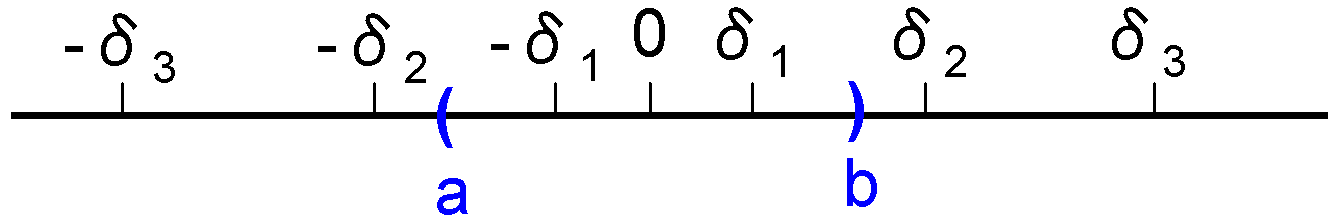
\includegraphics[height=0.4in,width=1.8in]{IncWiden.png} &
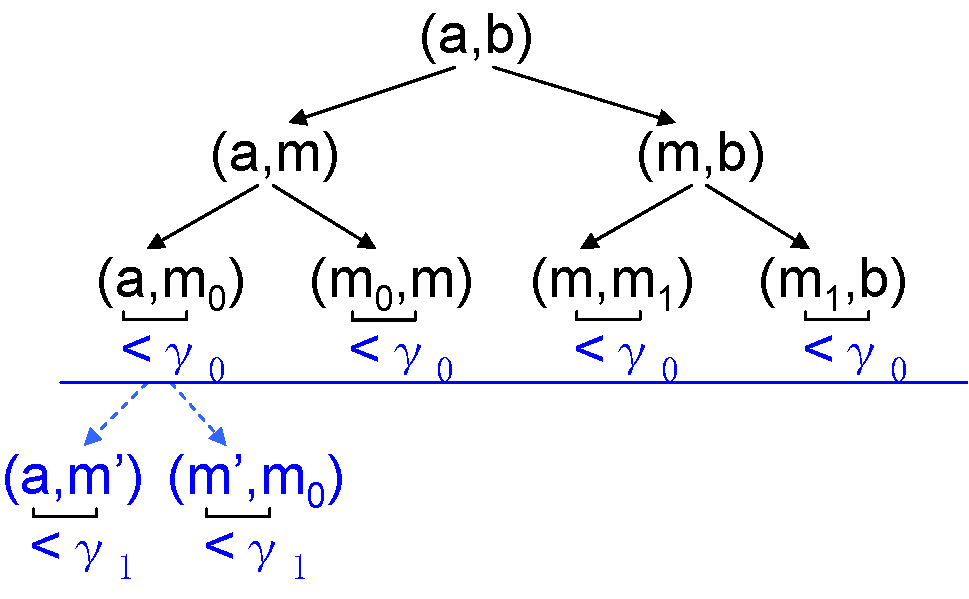
\includegraphics[height=1.2in,width=2in]{IncDeepen.png} \\
\mbox{(a) Incremental widening} & \mbox{(b) Incremental Deepening} \\
\end{tabular}
%\caption{Chebyshev approximation of $x^2$ and $x~|x|$}
\caption{Two incremental search strategies}
\label{fig:incwid}
\end{minipage}
\end{figure}


\subsubsection*{Incremental deepening}

To combine depth-first-search and breadth-first search among decomposed boxes,
{\bf raSAT} applied {\em incremental deepening}. 
Let $\gamma_0 > \gamma_1 > \cdots > 0$. 
It applies a threshold $\gamma$, such that no more decomposition occurs 
when a box becomes smaller than $\gamma$.
$\gamma$ is initially $\gamma=\gamma_0$. 
If neither SAT nor UNSAT is detected, {\bf raSAT} restarts with the threshold $\gamma_1$.
This continues until either SAT, timeout, or
a given bound of repeatation (Fig.~\ref{fig:incwid} (b)). 


\subsection{SAT directed heuristics measure} \label{sec:SATheuristics}

%%%
\suppress{
With several hundred variables, we observe that an SMT solver works
when either SAT, or UNSAT with small UNSAT core.
%
For the latter, we need an efficient heuristics to find an UNSAT core, which is left as future work. 
For the former, the keys are how to choose variables to decompose, and 
how to choose a box to explore.
}%%%

In {\bf raSAT}, a strategy to select a variable to decompose is in the following two steps. 
(1) First select a most likely influential {\em API}, and
(2) then choose a most likely influential variable in the selected API. 
For {\em most likely influential} measures, we apply the {\em SAT-likelihood} on APIs and
the {\em sensitivity} on variables, respectively. Note that the latter measure is defined
only by Affine Intervals. 

\sloppy

In line 3 of Algorithm~\ref{Al:raSATLoop}, we have a box $B$ and IA will estimate ranges of polynomials from $B$.
Let $range(g_j, B)$ be the estimated range of $g_j$ by IA. 
If IA is an Affine Interval,
we assume that the estimated range of $g_j$ has the form
${(c_1,d_1)\epsilon_1 + \cdots + (c_n,d_n)\epsilon_n}$.
By instantiating $(-1,1)$ to $\epsilon_i$, we obtain $range(g_j, B)$. 
%$(-1,1)$ for $i \in \{1, \cdots, n\}$. 
%and we can obtain $range(g_j, I'_1 \times \cdots \times I'_n)$ by
%instantiating $\epsilon_i$ with $(-1,1)$ for $i \in \{1, \cdots, n\}$. 
We define 
\begin{itemize} 
\item the {\em SAT-likelihood} of an API $g_j > 0$ by $| I \cap (0,\infty) | / |I|$
  for  $I = range(g_j, B)$, and 
\item the {\em sensitivity} of a variable $x_i$ in an API $g_j > 0$ by $max(|c_i|, |d_i|)$. 
\end{itemize} 

\begin{example} \label{examp:SATlikelihood}
In Example~\ref{examp:sensitivity}, 
\begin{itemize}
\item SAT-likelihood of $f$ is $0.4= \frac{6}{9-(-6)}$ by $AF_2$ 
and $0.36 = \frac{4.5}{4.5-(-8)}$ by $CAI$. 
\item the sensitivity of $x$ is $1$ by $AF_2$ and $3\frac{1}{4}$ by $CAI$,
  and that of $y$ is $2$ by both $AF_2$ and $CAI$. 
\end{itemize}
\end{example}


SAT-likelihood intends to estimate an API how likely to be SAT. 
%For choosing variables, {\bf raSAT} first choose a test-UNSAT API by SAT-likelihood. 
There are two choices on the SAT-likelihood, either {\em the largest} or {\em the least}. 
The {\em sensitivity} of a variable intends to estimate how a variable is influential
to the value of an API, and the largest sensitivity is considered to be the most influential. 
%From a selected API by SAT-likelihood, {\bf raSAT} selects a variable with the largest sensitivity. 
This selection of variables are used both for (1) {\em decomposition}, and 
(2) {\em test case generation}. 
For multiple test generation, we select multiple variables that have larger sensitivity. 

At the decomposition, {\bf raSAT} also examines the choice of the box.
We define the {\em SAT-likelihood} of a box $B$ by 
the least SAT-likelihood of APIs. 
Since the SAT-likelihood of each box is computed when it is created by the decomposition,
{\bf raSAT} simply compares newly decomposed boxes with the previous ones. 
There are two choices of boxes, 
(1) a box with the largest SAT-likelihood, and 
(2) a box with the largest number of SAT (concluded by either IA or Testing) APIs. 
These combinations of strategy choices are compared by experiments in Section~\ref{sec:experiment}. 


\subsubsection*{Test case generation strategy}
\sloppy
The sensitivity of variables is also used for test case generation.
That is, {\bf raSAT} generates two test cases for the specified number of variables,
and one for the rest. 
Such variables are selected from those with larger sensitivity.
When two test cases are generated, {\bf raSAT} also observes
the sign of the coefficients of noise symbols.
If positive, it takes the upper bound of possible values as the first test case; 
otherwise, the lower bound. The second test case is generated randomly. 

\begin{example}
  Let $g = -x_{15}*x_8+x_{15}*x_2-x_{10}*x_{16}0$ and consider a constraint $g > 0$. 
  For ${x_2 \in [9.9, 10]}, {x_8 \in [0, 0.1]}, {x_{10} \in [0, 0.1]}, {x_{15} \in [0, 10]},$ and
  $ x_{16} \in [0, 10]$, 
  ${0.25 \epsilon_2 - 0.25 \epsilon_8 - 0.25 \epsilon_{10} + 49.5\epsilon_{15} - 0.25\epsilon_{16}
    + 0.75\epsilon_{+-} + 49.25}$ is the estimated by $AF2$ for $g$.
  The coefficient of $\epsilon_2$ is $0.25$, which is positive. 
  Thus, if $x_2$ increases, the value of $g$ is likely to increase.
  Then, we take the upper bound of possible values of $x_2$ as a test case, i.e. $10$. 
  %As a result, the test case of $x_2$ is expected as high as possible in order to satisfy $g>0$.
  Similarly, we take the test cases for other variables: $x_8=0, x_{10}=0, x_{15}=10, x_{16}=0$, and 
  we have $g=100 > 0$ with them. 
\end{example}
\suppress{
I. Selecting API for Testing:
  (1) Difficulty first by SAT-likelihood.   
  (2) Easy first by SAT-likelihood
  (10) Random.,
II. Selecting Variable:
  (8) With sensitivity
  (9) Without sensitivity - Random: 
III. Selecting box:
  (3) SAT-directed using IA-Testing.
  (4) UNSAT-directed using IA-Testing.
  (5) SAT-directed using SAT-likelihood
  (6) UNSAT-directed using SAT-likelihood
  (7) Random
}

\section{Experiments} \label{sec:experiment}

%\subsection{{\bf raSAT} Implementation} 
We implement \textbf{raSAT} loop as an SMT solver {\bf raSAT}, 
based on MiniSat 2.2 as a backbone SAT solver and the library in \cite{Al2012.14} for
outward rounding in Interval Arithmetics. 
Various combinations of strategies of {\bf raSAT} (in Section~\ref{sec:strategy})
and random strategies are compared on {\em Zankl} and {\em Meti-Tarski} in NRA category 
and {\em AProVE} in NIA category from SMT-LIB. 
The best combination of choices are 
\begin{enumerate}
\item an test-UNSAT API  (API that cannot be satisfied by any test cases in Testing) choice by the least SAT-likelihood, 
\item a variable choice by the largest sensitivity, and 
\item a box choice by the largest SAT-likelihood. 
\end{enumerate} 
Sometimes a random choice of a test-UNSAT API (instead of the least SAT-likelihood) 
shows an equally good result. 
They are also compared with \textbf{Z3 4.3}, \textbf{iSAT3} and \textbf{dReal-2.15.01}
where the former is considered to be the state of the art~(\cite{Jovanovic13}), and 
the remaining ones are a popular ICP based tools. 
Note that our comparison in this section is only on polynomial inequality.
Preliminary results on equality will be reported in Section~\ref{sec:eq}. 
%Example~\ref{ex1} in Appendix~\ref{app:raSATexample} illustrates how {\bf raSAT} works. 
The experiments are with Intel Xeon E5-2680v2 2.80GHz and 4 GB of RAM. 


\subsection{Benchmarks from SMT-LIB} \label{sec:expsmtlib}

SMT-LIB\footnote{\tt http://www.smt-lib.org} 
benchmark on non-linear real number arithmetic 
(QF\_NRA) has Meti-Tarski, Keymaera, Kissing, Hong, and Zankl families,
of which brief statistics are summarized below. 
Until SMT-COMP 2011, benchmarks are only Zankl family. 
In SMT-COMP 2012, other families have been added, and currently growing. 
General comparison among various existing tools on these benchmarks is summarized in 
Table~1 in \cite{Jovanovic13}, which shows Z3 4.3 is one of the strongest. 

%From them, we extract problems of polynomial inequality only. %(not containing $''=''$). 
%The brief statistics and explanation are as follows. 
\begin{itemize}
\item {\bf Zankl} has 151 inequalities among 166, taken from termination provers. 
A problem may contain several hundred variables, an API may contain more than one hundred variables, 
and the number of APIs may be over thousands, though the maximum degree is up to $6$. 
\item {\bf Meti-Tarski} contains 5101 inequalities among 7713, taken from elementary physics.
They are mostly small problems, up to 8 variables (mostly up to 5 variables), and up to 20 APIs. 
\item {\bf Keymaera} contains 68 inequalities among 680. 
\item {\bf Kissing} has 45 problems, all of which contains equality (mostly single equation). 
%They are taken from the cases of touching curves. 
\item {\bf Hong} has 20 inequalities among 20, tuned for QE-CAD and quite artificial. 
\end{itemize}

The setting of the experiments are
\begin{itemize}
\item For test data generation, {\bf raSAT} chooses 10 variables (1 variable from each of 10 APIs
  with the largest SAT-likelihood) and generate 2 test cases for each of these, and single random test data is
  generated for each of the rest of variables.
\item For interval decomposition, {\bf raSAT} splits at exactly the middle. 
\end{itemize}


\subsection{Experiments on Strategy Combinations} \label{sec:expstrategy}

\subsubsection*{Selection of Incremental Strategies}
We run some options for incremental widening and incremental deepening on Zankl family
in order to select the best combination. From now on, we set as below. 
%Table~\ref{tab:incremental} 
\begin{itemize}
\item For incremental widening, $\delta_0 = 10, \delta_1 = \infty$.
\item For incremental deepening, $\gamma_i = 10^{-(i+1)}$ for $i = 0, 1, \cdots$
\end{itemize}

\begin{table}
\begin{center}
\adjustbox{max width=\columnwidth}{
\begin{tabular}{ | l | r | r | r | r  | r | r | r | r | r | r |r | r | r | r | r | r |}
\hline
    \multicolumn{1}{|l|}{Benchmark} & 
    \multicolumn{4}{c|}{$\delta_0 = \infty, \gamma_i=0.1$} & \multicolumn{4}{c|}{$\delta_0 = \infty, \gamma_i=10^{-(i+1)}$} & \multicolumn{4}{c|}{$\delta_0 = 10, \delta_1 = \infty, \gamma_i=10^{-(i+1)}$} & \multicolumn{4}{c|}{$\delta_0 = 1, \delta_1 = 10, \delta_3 = \infty, \gamma_i=10^{-(i+1)}$}\\
\hline
    & \multicolumn{2}{c}{SAT} & \multicolumn{2}{|c}{UNSAT} & \multicolumn{2}{|c}{SAT} 
    & \multicolumn{2}{|c}{UNSAT} & \multicolumn{2}{|c}{SAT} & \multicolumn{2}{|c}{UNSAT} & \multicolumn{2}{|c}{$\delta-$SAT} & \multicolumn{2}{|c|}{UNSAT}\\
\hline
Zankl& 4 & 5.75 (s) & 10 & 3.47 (s) & 5 & 6.16 (s) & 10 & 3.47 (s) & \textbf{20} & 244.34 (s) & 10 & 3.47 (s) & 2 & 205.64 (s) & 10 & 3.47 (s)\\
\hline
\end{tabular}
}
\end{center}
\caption{Options for Incremental Strategies} 
\label{tab:incremental}
\end{table}

%We perform experiments only on inequalities of Zankl, and Meti-Tarski families. 
Table~\ref{tab:rasat-experiments} shows the experimental results of above mentioned combination. 
The timeout is set to 500s, and time shows the total of successful cases 
(either SAT or UNSAT). Our combinations of strategies are,

\medskip
{\centering
\adjustbox{max width=\columnwidth}{
\begin{tabular}{l|l|l}
Selecting a test-UNSAT API~~ & Selecting a box (to explore): & 
Selecting a variable: \\  % (for Testing and decomposition)
\hline

(1) Least SAT-likelihood. & 
(3) Largest number of SAT APIs.~~ & 
(8) Largest sensitivity. \\

(2) Largest SAT-likelihood. & 
(4) Least number of SAT APIs. & \\

& (5) Largest SAT-likelihood. & \\

& (6) Least SAT-likelihood. & \\

(10) Random. & (7) Random. & (9) Random. \\
\end{tabular}
}
}
\noindent
where we randomly select points in the box $B$ (Algorithm~\ref{Al:raSATLoop}) as test cases in Testing. Here, (10)-(7)-(9) means all random selection. 
Generally speaking, the combination of (5) and (8) show the best results, 
though the choice of (1),(2), and (10) shows different behavior on benchmarks. 
We tentatively prefer (1) or (10), but it needs to be investigated further. 

\begin{table*}[t]
\centering
\adjustbox{max width=\columnwidth}{
\begin{tabular}{ | l | r | r | r | r  | r | r | r | r | r | r |r | r |}
\hline
    \multicolumn{1}{|l|}{Benchmark} & 
    \multicolumn{2}{c|}{(1)-(5)-(8)} & \multicolumn{2}{c|}{(1)-(5)-(9)} & 
    \multicolumn{2}{c|}{(1)-(6)-(8)} & \multicolumn{2}{c|}{(1)-(6)-(9)} &
    \multicolumn{2}{c|}{(10)-(5)-(8)} & \multicolumn{2}{c|}{(10)-(6)-(8)} 
\\
\hline
 Matrix-1 (SAT) & 20 & 132.72 (s) & 18 & 101.07 (s)& 15 & 1064.76 (s)& 14 & 562.19 (s)& \textbf{21} & 462.57 (s)& 18 & 788.46(s) 
\\
\hline
 Matrix-1 (UNSAT) & 2 & 0.01 (s)& 2 & 0.01 (s)&  2 & 0.01 (s)& 2 & 0.01 (s)& 2 & 0.01 (s)
& 2 & 0.01 (s)
\\
\hline
 Matrix-2,3,4,5 (SAT) & {\bf 10} & 632.37 (s)& 3 & 140.27 (s)& 1 & 3.46 (s)& 0 & 0.00 (s)& 5 & 943.08 (s)& 0 & 0.00 (s)
\\
\hline
 Matrix-2,3,4,5 (UNSAT) & 8 & 0.37 (s)& 8 & 0.39 (s)& 8 & 0.37 (s)& 8 & 0.38 (s)& 8 & 0.38 (s)& 8 & 0.38 (s)
\\
\hline
\hline
    \multicolumn{1}{|l|}{Benchmark} & 
    \multicolumn{2}{c|}{(2)-(5)-(8)} & \multicolumn{2}{c|}{(2)-(5)-(9)} & 
    \multicolumn{2}{c|}{(2)-(6)-(8)} & \multicolumn{2}{c|}{(2)-(6)-(9)} & 
    \multicolumn{2}{c|}{(2)-(7)-(8)} & \multicolumn{2}{c|}{(10)-(7)-(9)} \\
\hline
 Matrix-1 (SAT) & 20 & 163.47 (s) & 21 & 736.17 (s)& 19 & 953.97 (s)& 18 & 
1068.40 (s)& 19 & 799.79 (s)& 19 & 230.39 (s)
\\
\hline
 Matrix-1 (UNSAT) & 2 & 0.00(s) & 2 & 0.00 (s)& 2 & 0.00 (s)& 2 & 0.00 (s)& 2 & 0.00 (s)& 2 & 0.00 (s)
\\
\hline
 Matrix-2,3,4,5 (SAT) & 5 & 514.37 (s)& 1 & 350.84 (s)& 0 & 0.00 (s)& 0 & 0.00 (s)& 0 & 0.00 (s)& 1 & 13.43 (s)
\\
\hline
 Matrix-2,3,4,5 (UNSAT) & 8 & 0.43 (s)& 8 & 0.37 (s)& 8 & 0.40 (s)& 8 & 0.38 (s)& 8 & 0.37 (s)& 8 & 0.38 (s)
\\
\hline
\hline
    \multicolumn{1}{|l|}{Benchmark} & 
    \multicolumn{2}{c|}{(1)-(3)-(8)} & \multicolumn{2}{c|}{(1)-(4)-(8)} & 
    \multicolumn{2}{c|}{(2)-(3)-(8)} & \multicolumn{2}{c|}{(2)-(4)-(8)} & 
    \multicolumn{2}{c|}{(10)-(3)-(8)} & \multicolumn{2}{c|}{(10)-(4)-(8)} \\
\hline
 Matrix-1 (SAT) & 18 & 1438.47 (s) & 20 & 1537.9 (s)& 19 & 1100.60 (s)& 17 & 916.32 (s)& 17 & 87.78 (s)& 20 & 710.21 (s)
\\
\hline
 Matrix-1 (UNSAT) & 2 & 0.00 (s)& 2 & 0.00(s) & 2 & 0.00 (s)& 2 & 0.00 (s)& 2 & 0.00 (s)& 2 & 0.00 (s)
\\
\hline
 Matrix-2,3,4,5 (SAT) & 0 & 0.00 (s)& 1 & 33.17 (s)& 1 & 201.32 (s)& 2 & 328.03 (s)& 0 & 0.00 (s)& 1 & 20.94 (s)
\\
\hline
 Matrix-2,3,4,5 (UNSAT) & 8 & 0.36 (s)& 8 & 0.36 (s)& 8 & 0.34 (s)& 8 & 0.37 (s)& 8 & 0.37 (s)& 8 & 0.39 (s)
\\
\hline
\end{tabular}
}
\bigskip
\adjustbox{max width=\columnwidth}{
\begin{tabular}{ | l | r | r | r  | r | r | r | r | r |}
\hline
    \multicolumn{1}{|l|}{Benchmark} & 
    \multicolumn{2}{c|}{(1)-(5)-(8)} & \multicolumn{2}{c|}{(1)-(5)-(9)} & 
    \multicolumn{2}{c|}{(10)-(5)-(8)} & \multicolumn{2}{c|}{(10)-(7)-(9)} \\
\hline
    Meti-Tarski (SAT) & 3452 & 713.16 (s) & \textbf{3456} & 644.21 (s)& 3454 & 747.25 (s)& 3451 & 895.14 (s)
\\
\hline
    Meti-Tarski (UNSAT) & 1052 & 822.09 (s)& 1044 & 957.71 (s)& {\bf 1061} & 321.00 (s)& 1060 & 233.46 (s) 
\\
\hline
\end{tabular}
}
\medskip
\caption{Combinations of {\bf raSAT} strategies on NRA/Zankl,Meti-Tarski benchmark} 
\label{tab:rasat-experiments}
\end{table*}

%Experiments in Table~\ref{tab:rasat-experiments} are performed 
%with random generation ($k$-random tick) and the balanced decomposition 
%(dividing at the exact middle). 

\subsection*{Experiments with test case generation using variables sensitivity}
%From above section, we can see that the combination (1)-(5)-(8) shows the best performance on benchmarks.
This section examines the effectiveness of the sensitivity in test case generation, 
which is referred by (11).
Table~\ref{tab:test-sen} presents the result on Zankl and Meti-tarski
benchmarks, which show that this strategy made improvements in SAT detection. 

\begin{table}
\begin{center}
\begin{tabular}{ | l | r | r | r | r |}
\hline
    \multicolumn{1}{|l|}{Benchmark} & \multicolumn{2}{c|}{(1)-(5)-(8)} &
    \multicolumn{2}{c|}{(1)-(5)-(8)-(11)} \\
\hline
    Matrix-1 (SAT ) & 20 & 132.72 (s) & \textbf{25} & 414.99(s)
\\
\hline
    Matrix-1 (UNSAT) & 2 & 0.01(s) & 2 & 0.01(s)
\\
\hline
	Matrix-2,3,4,5 (SAT) & 10 & 632.37 (s) & \textbf{11} & 1264.77(s)
\\
\hline
    Matrix-2,3,4,5 (UNSAT) & 8 & 0.37(s) & 8 & 0.38(s)
\\ \hline
    Meti-Tarski (SAT) & 3452 & 713.16 (s) & \textbf{3473} & 419.25 (s)
\\
\hline
    Meti-Tarski (UNSAT) & 1052 & 822.09 (s) & 1052 & 821.85 (s)
\\
\hline
\end{tabular}
\end{center}
\caption{Effectiveness of variables sensitivity on test cases generation} 
\label{tab:test-sen}
\end{table}

\subsection{Comparison with other SMT solvers}

We compare {\bf raSAT} with other SMT solvers in Table~\ref{tab:comparison}.
%on NRA benchmarks: Zankl, Meti-Tarski and Keymaera. 
The timeout is $500s$. 
For {\bf iSAT3}, the ranges of all variables are uniformly set to be in the range $[-1000, 1000]$
(otherwise, it often causes segmentation fault). 
Thus, UNSAT detection of {\bf iSAT3} means UNSAT in the range $[-1000, 1000]$, 
while that of {\bf raSAT}, \textbf{dReal-2.15.01} and {\bf Z3 4.3} means UNSAT over $[-\infty, \infty]$.
Another note is that SAT statements by \textbf{dReal-2.15.01} means $\delta$-SAT, which allows
$\delta$ deviation. Thus, it does not mean really SAT, and a number of UNSAT problems in
Zankl, \textbf{dReal} concluded SAT.
%For instances, with a number of UNSAT problems in Zankl, \textbf{dReal} still concludes SAT.

Among these SMT solvers, {\bf Z3 4.3} shows the best performance. 
However, if we closely observe, there are certain tendency. 
{\bf Z3 4.3} is very quick for small constraints, i.e., with 
short APIs (up to $5$) and a small number of variables (up to $10$). 
{\bf raSAT} shows comparable performance on SAT detection with 
longer APIs (larger than $5$) and a larger number of variables (more than $10$), 
and sometimes outperforms on SAT detection of vary long constraints 
(APIs longer than $40$ and/or more than $20$ variables). 
Such examples appear in Zankl/matrix-3-all-*, matrix-4-all-*, and matrix-5-all-* 
(total 74 problems), and {\bf raSAT} solely solves 
\begin{itemize}
\item {\em matrix-3-all-2} (47 variables, 87 APIs, and max length of an API is 27), 
\item {\em matrix-3-all-5} (81 variables, 142 APIs, and max length of an API is 20), 
\item {\em matrix-4-all-3} (139 variables, 244 APIs, and max length of an API is 73), and 
\item {\em matrix-5-all-01} (132 variables, 276 APIs, and max length of an API is 47). 
\end{itemize}
Note that, for Zankl, when UNSAT is detected, it is detected very quickly. 
This is because SMT solvers find small UNSAT cores, without tracing all APIs.
Otherwise, it leads timeout. 
However, for SAT detection with large problems, 
SMT solvers need to trace all APIs. Thus, it takes much longer time. 

\begin{table*}[t]
\centering
\adjustbox{max width=\columnwidth}{
\begin{tabular}{ | l | r | r | r | r  | r | r | r | r | r | r |r | r | r | r | r | r |}
\hline
    \multicolumn{1}{|l|}{Benchmark} & 
    \multicolumn{4}{c|}{\bf raSAT} & \multicolumn{4}{c|}{\bf Z3 4.3} & \multicolumn{4}{c|}{\bf iSAT3} & \multicolumn{4}{c|}{\bf dReal}\\
\hline
    & \multicolumn{2}{c}{SAT} & \multicolumn{2}{|c}{UNSAT} & \multicolumn{2}{|c}{SAT} 
    & \multicolumn{2}{|c}{UNSAT} & \multicolumn{2}{|c}{SAT} & \multicolumn{2}{|c}{UNSAT} & \multicolumn{2}{|c}{$\delta-$SAT} & \multicolumn{2}{|c|}{UNSAT}\\
\hline
Zankl/matrix-1 (53) & 25 & 414.99 (s) & 2 & 0.01 (s) & \textbf{41} & 2.17 (s) & 12 & 0.00 (s) & 11 & 4.68 (s) & 3 & 0.00 (s) & 46 & 3573.43 (s) & 0 & 0.00 (s)\\
\hline
Zankl/matrix-2,3,4,5 (98) & 11 & 1264.77 (s) & 8 & 0.38 (s) & \textbf{13} & 1031.68 (s) & 11 & 0.57 (s) & 3 & 196.40 (s) & 12 & 8.06 (s) & 19& 2708.89 (s) & 0 & 0.00 (s) \\
\hline 
Meti-Tarski (5101) & 3473 & 419.25 (s) & 1052 & 821.85 (s) & \textbf{3528} & 51.22 (s) & 1568 & 78.56 (s) & 2916 & 811.53 (s) & 
1225 & 73.83 (s) & 3523 & 441.35 (s) & 1197 & 55.39 (s) \\
\hline
Keymaera (68) & 0 & 0.00 (s) & 16 & 0.06 (s) & 0 & 0.00 (s) & 68 & 0.36 (s) & 0 & 0.00 (s) & 
16 & 0.07 (s) & 8 & 0.18 (s) & 0 & 0.00 (s) \\
\hline
\end{tabular}
}
\medskip 
\caption{Comparison among SMT solvers over inequalities} \label{tab:comparison}
\end{table*}


\subsection{Polynomial Constraints Over Integers} \label{sec:NIA}

{\bf raSAT} loop is easily modified to QF\_NIA (nonlinear arithmetic over
integer numbers) from QF\_NRA.
We obtain SAT detection over integers by setting $\gamma_0 = 1$ in
the incremental deepening in Section~\ref{sec:incsearch} 
and restricting test data generation on integer numbers,
where UNSAT detection is the same as for QF\_NIA benchmarks. 
We compare {\bf raSAT} with {\bf Z3 4.3} on benchmarks of QF\_NIA/AProVE, 
which consists of 6850 inequalities and 1979 equalities. 
Some has several hundred variables, but each API has few variables
(mostly just 2 variables).
%Note that the use of the Intermediate Value Theorem cannot be applied
%for QF\_NIA constraints since the polynomials are not continuous.
%For SAT benchmarks (both inequalities and equalities), \textbf{raSAT}
%concludes satisfiability only by Testing.
The preliminary results (with the time out $500s$) are presented in
Table~\ref{tab:aprove}. 
\suppress{
\begin{itemize}
\item {\bf raSAT} detects 6773 SAT in 90.22s, and 2 UNSAT in 378.04s. 
\item {\bf Z3 4.3} detects 6784 SAT in 97.70s, and 36 UNSAT in 32.08s. 
\end{itemize}
where the timeout is $500s$. 
}
{\bf raSAT} does not detect UNSAT well since UNSAT problems
have quite large coefficients, which lead exhaustive search on quite large area.
\begin{table*}[t]
\centering
\begin{tabular}{ | l | r | r | r | r  | r | r | r | r |}
\hline
    \multicolumn{1}{|l|}{Benchmark} & 
    \multicolumn{4}{c|}{\bf raSAT} & \multicolumn{4}{c|}{\bf Z3 4.3}\\
\hline
    & \multicolumn{2}{c}{SAT} & \multicolumn{2}{|c}{UNSAT} 
    & \multicolumn{2}{|c}{SAT} & \multicolumn{2}{|c|}{UNSAT} \\
\hline
inequalities (6850) & \textbf{6784} & 65.60 (s) & 0 & 0.00 (s) &
\textbf{6784} & 97.77 (s) & \textbf{36} & 32.46 (s) 
\\
\hline
equalities (1979) & 891 & 33721.37 (s) & 16 & 27.34 (s) &
\textbf{900} & 1951.01(s) & \textbf{250} & 3104.74(s) 
\\
\hline
\end{tabular}
\medskip 
\caption{Comparison on NIA/AProVE} \label{tab:aprove}
\end{table*}


\section{Extension for Equality Handling} \label{sec:eq}

For a polynomial constraint with equality:
\[\varphi = \exists x_1 \in I_1 \cdots x_n \in I_n.
\bigwedge \limits_{j=1}^m \psi_j(x_1,\cdots,x_n) \wedge
\bigwedge \limits_{j=1}^{m'} g_j(x_1,\cdots,x_n) = 0\]
one typical way to solve equality is an algebraic method, e.g., Groebner basis.
In this section, we try a simple method based on
{\em Intermediate Value Theorem}. It is illustrated by a single equality case.
Note that before solving on equality, we assume a box
that makes $\bigwedge \limits_{j=1}^m \psi_j(x_1,\cdots,x_n)$ IA-valid. 

\subsubsection{Single Equality}
For solving polynomial constraints with single equality (${g=0}$),
we can apply in a simple way. 
That is, finding 2 test cases with $g > 0$ and $g < 0$ implies 
$g=0$ somewhere in between. 

\begin{lemma} \label{lemma:ivt}
For $\varphi = \exists x_1 \in I_1 \cdots x_n \in I_n
(\bigwedge \limits_{j=1}^m g_j > 0~\wedge~g = 0)$.
Suppose decomposition creates a box
$B = (l_1, h_1) \times \cdots \times (l_n, h_n)$
where $(l_i, h_i) \subseteq I_i$ for all $i \in \{1, \cdots, n\}$,
such that $\bigwedge \limits_{j=1}^m g_j > 0$ is IA-VALID in the box.
Let $(l_g, h_g) = range(g, B)$.
\begin{enumerate}[(i)]
\item If $l_g > 0$ or $h_g < 0$, then $F$ is UNSAT in the box. 
\item If there are two instances $\vec{t},\vec{t'}$ in the box
  with $g(\vec{t}) > 0$ and $g(\vec{t'}) < 0$, then F is SAT.
\end{enumerate}
\end{lemma}

%%%%%%%%%%%%%
\suppress{
\begin{proof}
\begin{enumerate}[(i)]
\item If $l_g > 0$ or $h_g < 0$, then $g=0$ cannot be satisfied in box $I$.
  As a result, $F$ is UNSAT in $I$. 
\item If there are two instances $\vec{t},\vec{t'}$ in the box with
  $g(\vec{t}) > 0$ and $g(\vec{t'}) < 0$, it is clear from the Intermediate
  Value Theorem that there exist one point $\vec{t_0}$ between $\vec{t}$ and
  $\vec{t'}$ such that $g(\vec{t_0}) = 0$. In addition, because
  $\bigwedge \limits_{j}^m f_j > 0$ is IA-VALID in $I$, $\vec{t_0}$ also
  satisfies $\bigwedge \limits_{j}^m f_j > 0$.
  As a result, $F$ is satisfiable with $\vec{t_0}$ as the SAT instance.
\end{enumerate}
\end{proof}
}
%%%%%%%%%%%%
If neither (i) nor (ii) holds, \textbf{raSAT} continues the decomposition.
\begin{example}
  Let $\varphi = f(x, y) > 0 \wedge g(x, y) = 0$.
  Suppose we find a box 
  ${B = (a, b) \times (c, d)}$
  such that $f(x, y) > 0$ is VALID in $B$.
  (Fig.~\ref{fig:single-equation}).
  In addition, inside the box,
  if we find two points $(u_1, v_1)$ and $(u_2, v_2)$ such that
  $g(u_1, v_1) > 0$ and $g(u_2, v_2) < 0$,
  then the constraint is satisfiable by Lemma~\ref{lemma:ivt}. 
\end{example}
\begin{figure}
\centering
\begin{subfigure}{0.49\textwidth}
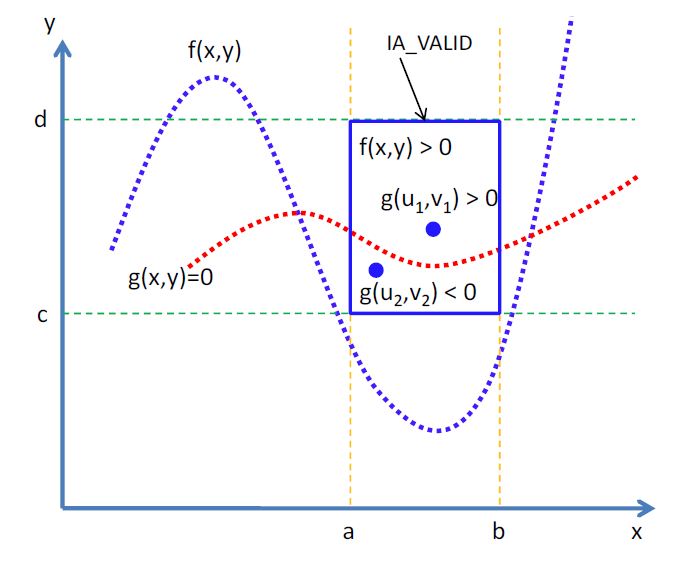
\includegraphics[width=1.\linewidth]{singleEquation.png} 
\caption{Single equality}
\label{fig:single-equation}
\end{subfigure}
\begin{subfigure}{0.49\textwidth}
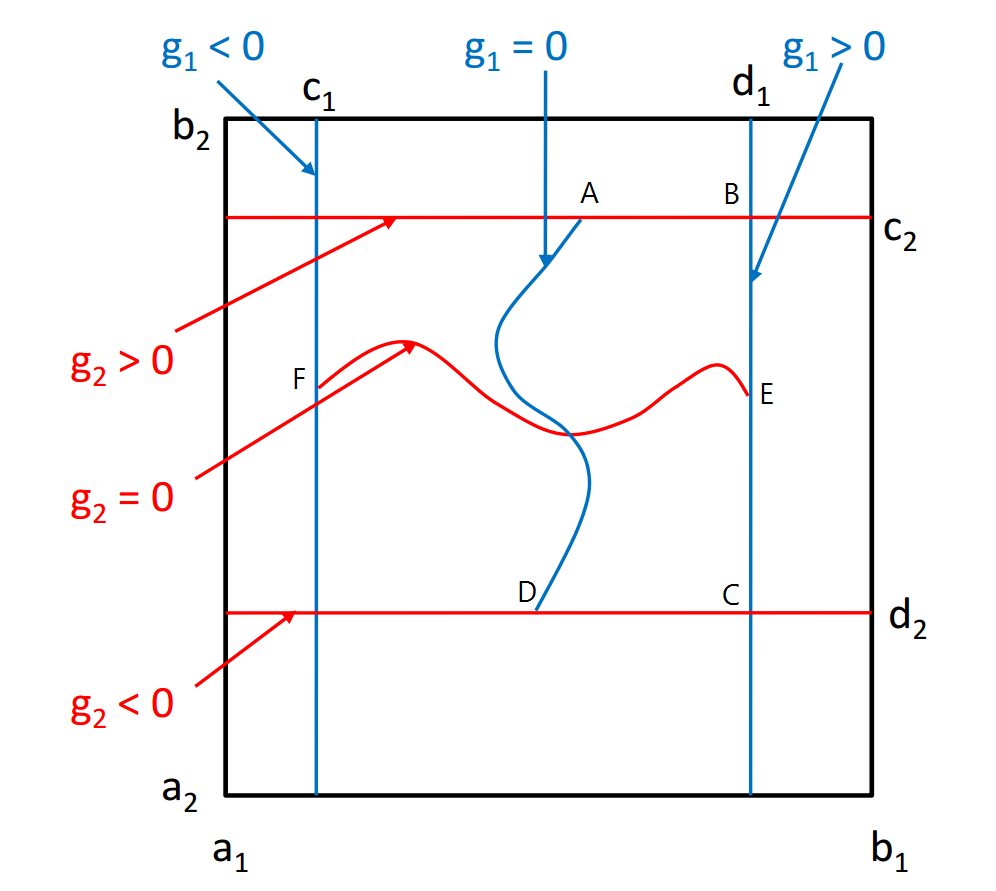
\includegraphics[width=1.\linewidth]{multipleEquations.png}  
\caption{Multiple equalities}
\label{fig:multiple-equations}  
\end{subfigure}
\caption{Example on solving equality using the Intermediate Value Theorem}
%\end{minipage}
\end{figure}
    {\bf raSAT} first tries to find a box (by the decomposition) such that
    $\bigwedge \limits_{j=1}^m g_j > 0$ is IA-VALID in the box.
    Then it tries to find 2 instances with $g > 0$ and $g < 0$ by Testing. 
    Intermediate Value Theorem guarantees the existence of an SAT instance
    in between. Note that this method does not find a SAT instance. 


\subsubsection{Multiple Equalities}
The idea of Intermediate Value Theorem is extended for solving multiple equalities. 
Consider $m$ equalities ($m \ge 1$): $\bigwedge \limits_{j=1}^m g_j = 0$ and 
an box $B = {(l_1, h_1) \times \cdots (l_n, h_n)}$.
For $V = \bigcup \limits_{j=1}^m var(g_j)$ and $V' = \{x_{j_1}, \cdots x_{j_k} \} \subseteq V$,
we denote $\{ (r_1, \cdots, r_n) \in B \mid r_i = l_i~\text{for }i=j_1,...,j_k \}$
and ${\{ (r_1, \cdots, r_n) \in B \mid r_i = h_i~\text{for }i=j_1,...,j_k \}}$
by $B\downarrow_{V'}$ and $B\uparrow_{V'}$, respectively. 

\begin{definition} \label{def:CheckBasis} 
A sequence $(V_1, \cdots, V_m)$ of subsets of $V$ is a {\em check basis} of $(g_1, \cdots, g_m)$ on a box $B$,
if, for each $j,j'$ with $1 \leq j, j' \leq m$, 
\begin{enumerate}
\item $V_j (\neq \emptyset) \subseteq var(g_j)$, 
\item $V_j \cap v_{j'} = \emptyset$ if $j \neq j'$, and 
\item either $g_j > 0$ on $B\uparrow_{V_j}$ and $g_j < 0$ on $B\downarrow_{V_j}$, or
      $g_j < 0$ on $B\uparrow_{V_j}$ and $g_j > 0$ on $B\downarrow_{V_j}$. 
\end{enumerate}
\end{definition} 
%%%
\suppress{
For all $j\in \{1, \cdots, m\}$, let $k_j = |V_j|$ and
${V_j = \{v_{jk} \mid 1 \le k \le k_j \}}$, then, there exist two combinations
${(x_{j1}, \cdots, x_{jk_j}) = (t_{j1}, \cdots, t_{jk_j})}$ and
${(x_{j1}, \cdots, x_{jk_j}) = (t'_{j1}, \cdots, t'_{jk_j})}$
where $t_{jk} \neq t'_{jk} \in (l_{jk}, h_{jk})$, $1 \le k \le k_j$ such that
\[g_j(t_{j1}, \cdots, t_{jk_j}, \cdots, x_{jk}, \cdots) > 0\] and
\[g_j(t'_{j1}, \cdots, t'_{jk_j}, \cdots, x_{jk}, \cdots) < 0\]
for all values of $x_{jk}$ in $(l_{jk}, h_{jk})$ where $x_{jk} \in var(g_j) \setminus V_j$.
We denote $ivt(g_j, V_j, I)$ to represent that the polynomial $g_j$ enjoy this property
with respect to $V_j$ and $I$.
} %%%

\begin{lemma} \label{lem:multieq}
For a polynomial constraint containing multiple equalities \[\varphi= \exists x_1 \in I_1 \cdots x_n \in I_n.
\bigwedge \limits_{j=1}^m \psi_j(x_1,\cdots,x_n) \wedge
\bigwedge \limits_{j=1}^{m'} g_j(x_1,\cdots,x_n) = 0\]
and a box $B \subseteq I_1 \times \cdots \times I_n$, 
assume that
\begin{enumerate}
\item $\bigwedge \limits_{j=1}^m \psi_j(x_1,\cdots,x_n)$ is IA-valid on $B$, and
\item there is a {\em check basis} $(V_1, \cdots, V_m)$ of $(g_1, \cdots, g_m)$ on B. 
\end{enumerate}
Then, $\bigwedge \limits_{j=1}^m g_j = 0$ has a SAT instance in $B$
(and thus $\varphi$ is SAT). 
\end{lemma}

The idea is, from the Intermediate Value Theorem,
each $g_j$ has a $n - |V_{j}|$ dimension surface of null points of $g_j$
between $B\uparrow_{V_j}$ and $B\downarrow_{V_j}$. 
Since $V_j$'s are mutually disjoint (and $g_j$' are continuous),
we have the intersection of all such surfaces of null points with
the dimension $n - \sum_{j=1}^m |V_j|$.
Thus, this method has a limitation that 
the number of variables must be greater than or equal to the number of equations.

\begin{example}
  Consider two equations $g_1(x, y)=0$ and $g_2(x, y) = 0$, and assume that $(\{x\}, \{y\})$
  is a check basis of $(g_1, g_2)$ on $(c_1,d_1) \times (c_2,d_2)$ (Fig.~\ref{fig:multiple-equations}).
  Then, the blue line (null points of $g_1$) and the red line (null points of $g_2$) must have
  an intersection. We can explain this by Jordan curve theorem. 
  Since $ABCD$ is a closed curve such that $E$ is inner and $F$ is outer,
  a continuous (red) line $EF$ must have an intersection by Jordan curve theorem. 
\end{example}

Current {\bf raSAT} implementation on equalities has only naive strategies. 
For instance, for each $g_j = 0$, \textbf{raSAT} checks all possible subsets of its variables
as candidates for $V_j$. Thus, in the worst case \textbf{raSAT} checks
$2^{|var(g_1)|}*\cdots*2^{|var(g_m)|}$ cases.
It also does not prepare a strategy to find a box that makes all inequalities IA-valid.
Preliminary experiments on equalities from QF\_NRA/Zankl and QF\_NRA/Meti-tarski
are summarized in Table~\ref{tab:equations}.
We hope that the sensitivity will give their effective strategies. 
\begin{table*}[t]
\centering
\adjustbox{max width=\columnwidth}{
\begin{tabular}{ | l | r | r | r | r  | r | r | r | r | r | r |r | r | r | r | r | r |}
\hline
    \multicolumn{1}{|l|}{Benchmark} & 
    \multicolumn{4}{c|}{\bf raSAT} & \multicolumn{4}{c|}{\bf Z3 4.3} & \multicolumn{4}{c|}{\bf iSAT3} & \multicolumn{4}{c|}{\bf dReal}\\
\hline
    & \multicolumn{2}{c}{SAT} & \multicolumn{2}{|c}{UNSAT} & \multicolumn{2}{|c}{SAT} 
    & \multicolumn{2}{|c}{UNSAT} & \multicolumn{2}{|c}{SAT} & \multicolumn{2}{|c}{UNSAT} & \multicolumn{2}{|c}{$\delta-$SAT} & \multicolumn{2}{|c|}{UNSAT}\\
\hline
Zankl (15) & \textbf{11} & 0.07 (s) & \textbf{4} & 0.17 (s) & \textbf{11} & 0.17 (s) & \textbf{4} & 0.02 (s) & 0 & 0.00 (s) & \textbf{4} & 0.05 (s) & 11 & 0.06 (s) & \textbf{4} & 0.02(s)\\
\hline
Meti-Tarski (3528/1573) & 875 & 174.90 (s) & 781 & 401.15 (s) & \textbf{1497} & 21.00 (s) & \textbf{1115} & 74.19 (s) & 1 & 0.28 (s) & 
1075 & 22.6 (s) & 1497 & 72.85 (s) & 943 & 21.40 (s) \\
\hline
Keymaera (612) & 0 & 0.00 (s)& 312 & 66.63 (s) & 0 & 0.00 (s) & \textbf{610} & 2.92 (s) & 0 & 0.00 (s) & 226 & 1.63 (s) & 13& 4.03 (s) & 318 & 1.96 (s) \\
\hline 
\end{tabular}
}
\medskip 
\caption{Comparison among SMT solvers with equations} \label{tab:equations}
\end{table*}


%%%%%%
\suppress{
\begin{algorithm}
\begin{algorithmic}[1]
\Function{equationsProver}{$\bigwedge\limits_{j=k}^mg_j = 0, \Pi, V_0$}
\If {$k > m$} \Comment{All equations are checked}
	\State \Return SAT
\EndIf
\For {$V_k \in P(var(g_k))$} \Comment{$P(var(g_k))$ is the powerset of $var(g_k)$}
	\If {$V_k \cap V = \emptyset$ and $ivt(g_k, V_k, \Pi)$}
		\State $V_0 \gets V_0 \cup V_k$
		\If {\Call{equationsProver}{$\bigwedge\limits_{j=k+1}^mg_j = 0, \Pi, V_0$} = SAT}
			\State \Return SAT
		\EndIf
	\EndIf
\EndFor
\State \Return UNSAT
\EndFunction
\State \Call{equationsProver}{$\bigwedge\limits_{j=1}^mg_j = 0, \Pi, \emptyset$}
\end{algorithmic}
\caption{Solving multiple equations $\bigwedge\limits_{j=1}^m g_j = 0$ with interval constraint ${\Pi = \bigwedge\limits_{i = 1}^n x_i \in (l_i, h_i)}$}
\label{Al:multiple-equations}
\end{algorithm}
}%%%%%%



%%%%%%%%%%%%%%%%%
\suppress{
\section{Equality handling} \label{sec:equality}

\subsection{Greater-than-or-Equal Handling} \label{sec:geq}

{\bf raSAT} loop is designed to solve polynomial inequality. 
There are several ways to extend to handle equality, in which our idea shares similarity with 
dReal~\cite{dRealCADE13,dRealLICS12}. 

\begin{definition} \label{def:strict_unsat}
$\bigwedge \limits_{j} f_j \geq 0$ is 
{\em strict-SAT} (resp. {\em strict-UNSAT}) 
if $\bigwedge \limits_{j} f_j > \delta_j$ is SAT 
(resp. $\bigwedge \limits_{j} f_j > -\delta_j$ is UNSAT) for some $\delta_j >0$.
\end{definition}

\begin{lemma} \label{lem:strict_sat}
If $\bigwedge \limits_{j} f_j \geq 0$ is {\em strict-SAT} (resp. {\em strict-UNSAT}), 
it is SAT (resp. UNSAT).
\end{lemma}

Note that netiher strict-SAT nor strict-UNSAT (i.e., kissing situation), 
%if $\bigwedge \limits_{j} f_j \geq 0$ is SAT but $\bigwedge \limits_{j} f_j > 0$ is UNSAT 
Lemma~\ref{lem:strict_sat} cannot conclude anything, and \textbf{raSAT} says {\em unknown}. 
%In implementation of \textbf{raSAT}, when $\geq$ appears, exploration of IA-SAT 
%(resp. IA-UNSAT) is reduced to that of IA-strict-SAT (resp. IA-strict-UNSAT). 


\subsection{SAT on Equality by Intermediate Value Theorem} \label{sec:eq}
For solving polynomial constraints with single equality ($g=0$), we apply {\em Intermediate Value Theorem}. 
That is, if existing 2 test cases such that $g > 0$ and $g < 0$, then $g=0$ is SAT somewhere in between, 
as in Fig.~\ref{fig:ivt}. 

\begin{lemma} \label{lemma:ivt}
For $F = \exists x_1 \in (a_1,b_1) \wedge \cdots \wedge x_n \in (a_n,b_n). 
\bigwedge \limits_{j}^m f_j > 0~\wedge~g = 0$, $F$ is SAT, if 
there is a box $(l_1, h_1) \times \cdots \times (l_n,h_n)$ with $ (l_i,h_i) \subseteq (a_i,b_i)$ 
such that 
\begin{enumerate}[(i)]
\item $\bigwedge \limits_{j}^m f_j > 0$ is IA-VALID in the box, and 
\item there are two instances $\vec{t},\vec{t'}$ in the box with $g(\vec{t}) > 0$ and $g(\vec{t'}) < 0$.
\end{enumerate}
\end{lemma}

{\bf raSAT} first tries to find an IA-VALID box for $\bigwedge \limits_{j}^m f_j > 0$ by refinements. 
If such a box is found, it tries to find 2 instances for $g > 0$ and $g < 0$ by Testing. 
Intermediate Value Theorem guarantees the existence of an SAT instance in between. 
Note that this method works for single equality and does not find an exact SAT instance. 
If multiple equalities do not share variables each other, we can apply Intermediate Value Theorem 
repeatedly to decide SAT. In Zankl benchmarks in SMT-lib, there are 15 gen-**.smt2 that contain equality
(among 166 problems), and each of them satisty this condition. 


 
\suppress{
In Table \ref{tab:eqexp} we show preliminary experiment for 15 problems that contain polynomial equalities in Zankl family. \textbf{raSAT} works well for these SAT problems and it can detect all SAT problems (11 among 15). At the current implementation, raSAT reports \emph{unknown} for UNSAT problems. The first 4 columns indicate \emph{name of problems}, \emph{the number of variables}, \emph{the number of polynomial equalities} and \emph{the number of inequalities}  in each problem, respectively. The last 2 columns show comparison results of \textbf{Z3 4.3} and \textbf{raSAT}.
\begin{table}
\centering
\scalebox{1.0}{
\begin{tabular}[b]{|c|c|c|c|c|c|c|c|}
\hline
%\multirow{2}{*}{Problem} & {No.} & {No.} & {No.}&
{Problem} & {No.} & {No.} & {No.}&
\multicolumn{2}{c|}{\textbf{Z3 4.3} (15/15)} &\multicolumn{2}{c|}{\textbf{raSAT} (11/15)}\\
\cline{5-8}
Name & Variables& Equalities& Inequalities&{Result} & {Time(s)}&{Result} & {Time(s)}\\
\hline
gen-03 & 1 & 1 & 0& SAT &0.01 & SAT &0.015\\
\hline
gen-04 & 1 & 1 & 0& SAT &0.01 & SAT &0.015\\
\hline
gen-05 & 2 & 2 & 0& SAT &0.01 & SAT &0.046\\
\hline
gen-06 & 2 & 2 & 1& SAT &0.01 & SAT &0.062\\
\hline
gen-07 & 2 & 2 & 0& SAT &0.01 & SAT &0.062\\
\hline
gen-08 & 2 & 2 & 1& SAT &0.01 & SAT &0.062\\
\hline
gen-09 & 2 & 2 & 1& SAT &0.03 & SAT &0.062\\
\hline
gen-10 & 1 & 1 & 0& SAT &0.02 & SAT &0.031\\
\hline
gen-13 & 1 & 1 & 0& UNSAT &0.05 & unknown &0.015\\
\hline
gen-14 & 1 & 1 & 0& UNSAT &0.01 & unknown &0.015\\
\hline
gen-15 & 2 & 3 & 0& UNSAT &0.01 & unknown &0.015\\
\hline
gen-16 & 2 & 2 & 1& SAT &0.01 & SAT &0.062\\
\hline
gen-17 & 2 & 3 & 0& UNSAT &0.01 & unknown &0.031\\
\hline
gen-18 & 2 & 2 & 1& SAT &0.01 & SAT &0.078\\
\hline
gen-19 & 2 & 2 & 1& SAT &0.05 & SAT &0.046\\
\hline
\end{tabular}
}
\caption{Experimental results for 15 equality problems of Zankl family}
\label{tab:eqexp}
\end{table}

We also apply the same idea for multiple equalities $\bigwedge \limits_{i} g_i = 0$ such that $Var(g_k) \cap Var(g_{k'}) = \emptyset$ where $Var(g_k)$ is denoted for the set of variables in the polynomial $g_k$. In the next section we will present idea for solving general cases of multiple equalities.
}

}
%%%%%%%%%%%%%%%%%%%%%%%%%%%%%


\section{Related Work} \label{sec:relate}

Non-linear constraints are still under ivestigation, and many techniques appear in SMT solvers. 

\begin{description}
\item[QE-CAD] RAHD \cite{Passmore09combineddecision} and 
Z3 4.3 (nlsat in~\cite{Jovanovic13}) include QE-CAD. 
%such as QEPCAD-B, Reduce/Redlog, and Mathematica. 
%QE-CAD is precise and detects beyond SAT instances (e.g., SAT regions), 
%scalability is still challenging, since it is DEXPTIME. 
%Since QE-CAD is DEXPTIME wrt the number of variables, 

\item[Virtual substitution (VS)]
%Virtual substitution is an EXPTIME algorithm 
%applicable when the degree of each variable does not exceed 4. 
SMT-RAT toolbox \cite{smtrat} combines 
VS, incremental DPLL, and %less lazy and 
eager theory propagation. 
Z3 3.1 %, the winner of QF\_NRA in SMT competition 2011, 
combines VS, ICP, and linearization.

\item[Bit-blasting] %Bit-blasting in bounded bit width is often used in SMTs for QF\_NIA. 
UCLID~\cite{Bryant07decidingbit-vector} and MiniSmt~\cite{Zankl:2010:SNR:1939141.1939168} give a bound on the number of bits 
%(i.e., narrowing bounds for SAT instances) 
%as an under-approximation, and removes clauses as an over-approximation. 
%They refine each other, which shares a similar sprit with {\bf raSAT} loop. 
%the winner of QF\_NRA in SMT competition 2010, 
%applies it 
to encode integers and rationals, respectively. %with symbolic representations for prefixed algebraic numbers. 
%MiniSmt can show SAT quickly with small degree polynomials, but due to the bounded bit encoding, 
%it cannot conclude UNSAT.
%Bit-blasting also suffers a lot when the degree of polynomials increases. 

\item[Linearization] %Linearization of polynomials is often used over integers, such as
%Barcelogic~\cite{Borralleras:2009:SNP:1614530.1614561}, 
%substitutes all possible integers in a given-bound to an argument of a multiplication. 
%Then, multiplications are reduced to an exhaustive search on linear constraints. 
CORD \cite{cordic} %uses another 
linearizes multiplications of reals by CORDIC encoding. 
%Both Barcelogic and CORD apply Yices for solving linear constraints.
Linearization suffers from the increase of the polynomial degrees. 
%\mizuhito{Check CORD is whether bit-blasting or linearization}. 
\end{description}


ICP-based SMT solvers are \text{iSAT3} and \text{dReal}, adding to \textbf{raSAT}. 
%Because \textbf{raSAT} in the same category of using ICP with 
%next part is going to take a look at details of methodologies used in these solvers.
\begin{description}
\item[iSAT3] It has tighter integration between DPLL procedure~\cite{dpll} and ICP. 
Fresh variables are introduced to decompose a polynomial to atomic representations, 
and each of them is assigned to an atomic proposition. 
A special data structure is prepared to store intervals such that 
they correspond to the decision level one in DPLL. 
Its unit propagation is strengthened by combining with eager theory propagation. 
In a clause, if all except one literals are falsified, the remaining literal causes unit propagation 
and it becomes a candidate when next decomposition occurs. 
Note that \textbf{iSAT3} uses only CI as an interval arithmetic. 

\item[dReal] It has different judgements on SAT, called $\delta$-SAT, which allows the deviation of the width $\delta$. 
Thus, $\delta$-SAT does not imply really SAT. This is the reason why dReal quite often concludes SAT (actually $\delta$-SAT) 
for UNSAT problems in SMT-comp benchmarks. With the weaking of SAT to $\delta$-SAT, it obtains the completeness of 
$\delta$-SAT and $\delta$-UNSAT~\cite{Gao:2012:9DP:2352896.2352921}. 
Note that \textbf{dReal} uses only CI as an interval arithmetic, and lazy theory propagation as {\bf raSAT}. 
\end{description}

%%%%%%%%%%%%%%%%%%%%%%%%%%%%%
\suppress{
\subsection*{iSAT3}
Although \textbf{iSAT3} also uses Interval Arithmetic (IA), its algorithm integrates IA with 
DPLL procedure~\cite{dpll} tighter than that of \textbf{raSAT}. 
During DPLL procedure, in addition to an assignment of literals, \textbf{iSAT3} also prepares 
a data structure to store interval boxes where each box corresponds to one decision level of DPLL procedure's assignment. 
In \textbf{UnitPropagation} rule, intead of using standard rule, 
\textbf{iSAT3} searches for clauses that have all but one atoms being inconsistence with the current interval box. 
When some atom are selected for the literals assignment, this tool tries to use the selected atoms to contract 
the corresponding box to make it smaller. In order to do this, \textbf{iSAT3} convert each inequality/equation 
in the given constraints into the conjunction of the atoms of the following form by introducing additional variables:
\begin{center}
\begin{tabular}{l c l}
atom &::=& bound $\mid$ equation \\
bound &::=& variable relation rational\_constant \\
relation &::=& $< \mid \le \mid = \mid \ge \mid >$ \\
equation &::=& variable = variable bop variable \\
bop &::=& $+ \mid - \mid \times$
\end{tabular}
\end{center}
In other words, the resulting atoms are of the form, e.g., either $x > 10$ or $x = y + z$. 
For example, the constraint \[x^2 + y^2 < 1\] is converted into:
\[\left\{ 
  \begin{array}{l}
    x_1 = x^2\\
    x_2 = y^2\\
    x_3 = x_1 + x_2\\
    x_3 < 1
   \end{array}
    \right.\]
From the atoms of these form, the contraction can be easily done for interval boxes:
\begin{itemize}
\item[$\bullet$] For the bound atom of the form, e.g., $x > 10$, if the bound is $x \in [0, 100]$, 
then the contracted box contain $x \in [10, 100]$.
\item[$\bullet$] For the equations of three variables $x = y \text{ bop } z$, from bounds of any two variables, 
we can infer the bound for the remaining one. For example, from
\[\left\{ 
  \begin{array}{l}
    x = y.z\\
    x \in [1, 10]\\
    y \in [3, 7]\\
   \end{array}
    \right.\]
we can infer that \[z \in [\frac{1}{7}, \frac{10}{3}] \]
\end{itemize}
When the \textbf{UnitPropagation} and contraction can not be done, \textbf{iSAT3} split one interval (decomposition) 
in the current box and select one decomposed interval to explore which corresponds to \textbf{decide} step. 
If the contraction yields an empty box, a conflict is detected and the complement of the bound selection 
in the last split needs to be asserted. This is done via \textbf{learn} the causes of the conflict and 
\textbf{backjump} to the previous bound selection of the last bound selection. In order to reason about causes of a conflict, 
\textbf{iSAT3} maintains an implication graph to represents which atoms lead to the asserting of one atom. 

\subsection*{dReal}
In stead of showing satisfiability/unsatisfiability of the polynomial constraints $\varphi$ over reals, 
\textbf{dReal} proves that either
\begin{itemize}
\item [$\bullet$] $\varphi$ is unsatisfiable, or 
\item [$\bullet$] $\varphi^\delta$ is satisfiable. 
\end{itemize}
Here, $\varphi^\delta$ is the $\delta$-weakening of $\varphi$. For instance, the $\delta$-weakening of $x = 0$ is 
$|x| \le \delta$. Any constraint with operators in $\{<, \le, > , \ge, =, \not=\}$ can be converted into constraints 
that contains only $=$ by the following transformations.
\begin{itemize}
\item [$\bullet$] \textbf{Removing $\not=$}: Each formula of the form $f \not= 0$ is transformed into $f > 0 \vee f < 0$.
\item [$\bullet$] \textbf{Removing $<$ and $\le$}: Each formula of the form $f < 0$ or $f \le 0$ is transformed into 
$-f \ge 0$ or $-f > 0$ respectively.
\item [$\bullet$] \textbf{Removing $>$ and $\ge$}: Each formula of the form $f > 0$ or $f \ge 0$ is transformed into 
$f - x = 0$ by introducing an auxiliary variable $x$ that has bound $[0, m]$ or $(0, m]$ respectively. 
Here, $m$ is any rational number which is greater than the maximum of $f$ over intervals of variables. 
As the result, \textbf{dReal} requires the input that ranges of variables must be compact.
\end{itemize}

Note that the satisfiability of $\varphi^\delta$ does not imply that of $\varphi$. 
\textbf{dReal}'s methodology~\cite{Gao:2012:9DP:2352896.2352921} also cooperates DPLL with ICP 
in the lazy manner as in \textbf{raSAT}.

\medskip 
%{\bf raSAT} applies SAT confirmation to avoid soundness errors caused by roundoff/overflow errors. 
%Another static analysis based approach is found in~\cite{SilvaTACAS12}. 
}
%%%%%%%%%%%%%%%%%%%%%%%%%%%%%

%\subsection{Future Work}
%
\section{Conclusion} \label{sec:conclusion and Future Work}


This paper presented {\bf raSAT} loop, which extends ICP with Testing to accelerate
SAT detection and implemented as an SMT solver \textbf{raSAT}. With experiments on benchmarks from QF NRA category of SMT-lib, we found two heuristic measures SAT-likelihood and sensitivity, which lead effective strategy combination for SAT detection.
{\bf raSAT} still remains in naive proto-type status, and 
there are lots of future work. 

\medskip \noindent 
{\bf UNSAT core}. Currently, \textbf{raSAT} focuses on SAT detection. For
UNSAT detection, the target is to find a small UNSAT core in a large problem.


\medskip \noindent 
{\bf Equality handling}. 
Section~\ref{sec:eq} shows equality handling where UNSAT constraints can be completely solved by ICP (with the assumption of bounded intervals). The Intermediate Value Theorem can be used to show satisfiability with restrictions on variables of polynomials. Moreover, the use of this theorem is not complete in showing satisfiability. As a future work, we will apply Groebner basis in addition to the current use of the Intermediate Value Theorem.

\medskip \noindent 
{\bf Further strategy refiment}. 
Currently, raSAT uses only information from Interval Arithmetic .We are planning to refine strategies such that previous
IA and Testing results mutually guide to each other. For instance, a box decomposition strategy can be more focused.

%%%
\suppress{
\subsubsection{Extension of {\bf raSAT} loop}
\begin{itemize}
\item {\bf Equality handling}: currently, {\bf raSAT} loop can handle only inequalities. 
Before applying ideal based technique, such as {\em Gr{\"o}bner basis}, 
we are planning to implement a non-constructive detection of equality 
by {\em intermediate value theorem}. 

\suppress{
\item{\textbf{Polynomial equality by Intermediate value theorem}:} 
Consider 
\begin{center}
$(x_1 \in (a_1,b_1) \wedge \cdots \wedge x_n \in (a_n,b_n))~\bigwedge 
\limits_{j}^m f_j(x_1,\cdots,x_n) > 0~\wedge~g(x_1,\cdots, x_n) = 0.$
\end{center}
SAT can be proved by two steps. First, find a box of the product of 
$(l_{ik},h_{ik}) \subseteq (l_i,h_i)$ (by Interval Arithmetic) such that 
\begin{center}
$\forall x_1 \in (l_{1k},h_{1k}) \cdots x_n \in (l_{nk},h_{nk}).~\bigwedge 
 \limits_{j}^m f_j(x_1,\cdots,x_n) > 0$~~~~(IA-VALID) 
\end{center}
and find two instances (by Testing) in the box with $g(a_1,\cdots,a_n) > 0$ 
and $g(b_1,\cdots,b_n) < 0$. By Intermediate value theorem, we can conclude 
$\exists x_1 \in (l_1,h_1) \cdots x_n \in (l_n,h_n).~g(x_1,\cdots, x_n) = 0$. 
}

\item \textbf{Solving polynomial constraints on integers}: 
In integer domain, the number of test data is finite if interval constraints are bounded. 
Then, Test-UNSAT implies UNSAT if all possible test data are generated. 
A tight interaction between Testing and interval decomposition could be investigated.
Mixed integers are also challenging. 
\end{itemize}


\subsubsection{\textbf{raSAT} Development}

\begin{itemize}
\item \textbf{Avoiding local optimal}: 
we borrow an idea of \emph{restart} in MiniSAT for escaping from hopeless local search 
(i.e., solution set is not dense or empty). 
\emph{Heuristics} would be, after a deep interval decomposition of 
a box and Test-UNSAT are reported, backtrack occurs to choose a randomly selected box. 

\item \textbf{Separation of linear constraints}: 
Many benchmarks contain linear constraints. Current implementation does not have 
any tuning, but {\bf raSAT} loop only. 
Practically, separating linear and non-linear constraints and solving them 
in a coordinated way between Presbuger arithmetic and {\bf raSAT} would improve. 
During this separation, variables of intersecting linear constraints would be candidates 
for interval decompositions. 

\item \textbf{Incremental DPLL}: For interactions with the SAT solver, 
we currently apply the very lazy theory learning. Combination with 
\emph{eager} theory propagation would improve, in which we can propagate 
a conflict from a partial truth assignment instead of waiting 
for a full truth assignment obtained by SAT solver.
\end{itemize}
}
%%

%%
\suppress{
\subsection{Applications}
\begin{itemize}
\item \textbf{Checking overflow and roundoff error}: In the computers, the real numbers are represented by finite numbers (i.e., floating point numbers, fixed point numbers). Due to finite representation, the over-flow and roundoff errors (OREs) \cite{ngocsefm, ngocase} may occur. The OREs will be propagated through computations of the program. Further, the computations themselves also cause OREs because the arithmetic needs to round the result to fit the number format. Besides, OREs are also affected by types of statements, i.e., branch, loop, assignment statements.
By symbolic execution, ORE constraints are propagated from a program and ORE problems are reduced to problems of solving ORE constraints for verifying whether OREs occur. 
%For solving ORE constraint, combination of the new form of affine arithmetic ($CAI_1$) and \emph{sensitivity} (i.e., high degrees, )

\item \textbf{Loop invariant generation}: The problem of linear invariant generation is often reduced to the problem of non-linear constraint solving. 
Since Farkas's Lemma \cite{Colon03} uses the product of matrices with polynomial constraint solving, we can extend the target for non-linear invariant generation.
%Based on Farkas' Lemma \cite{Colon03}, non-linear constraints on coefficients of the target linear invariant are generated and a satisfiable instance of these constraints is a candidate of the linear invariant. 
\end{itemize}
}
%%


%\balance
\bibliographystyle{splncs03}
%\bibliography{generic}
\begin{thebibliography}{10}
\providecommand{\url}[1]{\texttt{#1}}
\providecommand{\urlprefix}{URL }

\bibitem{Al2012.14}
Alliot, J.M., Gotteland, J.B., Vanaret, C., Durand, N., Gianazza, D.:
  {Implementing an interval computation library for OCaml on x86/amd64
  architectures}. {ICFP}, ACM (2012)

\bibitem{benhamou:hal-00480814}
Benhamou, F., Granvilliers, L.: {Continuous and Interval Constraints}. {Handbook of Constraint Programming} (2006), pp.
  571--604

\bibitem{Bryant07decidingbit-vector}
Bryant, R.E., Kroening, D., Ouaknine, J., Seshia, S.A., Strichman, O., Brady,
  B.: Deciding bit-vector arithmetic with abstraction. TACAS 2007.
  LNCS 4424, pp. 358--372 (2007)

\bibitem{qecad}
Collins, G.: Quantifier elimination by cylindrical algebraic decomposition - twenty years of progress. Quantifier Elimination and Cylindrical
  Algebraic Decomposition, pp. 8--23 (1998)

\bibitem{Colon}
Colón, M., Sankaranarayanan, S., Sipma, H.: Linear invariant generation using
  non-linear constraint solving. 
  CAV, LNCS 2725, pp. 420--432
  (2003)
  
\bibitem{Comba93affinearithmetic}
Comba, J.L.D., Stolfi, J.: Affine arithmetic and its applications to computer
  graphics (1993)

\bibitem{smtrat}
Corzilius, F., Loup, U., Junges, S., Ábrahám, E.: Smt-rat: An smt-compliant
  nonlinear real arithmetic toolbox. SAT 2012, vol. 7317, pp. 442--448

\bibitem{isat}
Fränzle, M., Herde, C., Teige, T., Ratschan, S., Schubert, T.: Efficient
  solving of large non-linear arithmetic constraint systems with complex
  boolean structure. JSAT 1,  209--236 (2007)

\bibitem{cordic}
Ganai, M., Ivancic, F.: Efficient decision procedure for non-linear arithmetic
  constraints using cordic.
  FMCAD 2009. pp. 61--68 (2009).

\bibitem{Gao:2012:9DP:2352896.2352921}
Gao, S., Avigad, J., Clarke, E.M.: Delta-complete decision procedures for
  satisfiability over the reals. IJCAR'12, pp. 286--300 (2012)

\bibitem{dRealCADE13}
Gao, S., Kong, S., Clarke, E.: dreal: An smt solver for nonlinear theories over
  the reals. CADE-24, LNCS 7898, pp. 208--214 (2013)

\bibitem{Hickey:2001:IAP:502102.502106}
Hickey, T., Ju, Q., Van~Emden, M.H.: Interval Arithmetic: From principles to
  implementation. J. ACM  48(5),  1038--1068 (Sep 2001)

\bibitem{Hong2012883}
Hong, H., Din, M.S.E.: Variant quantifier elimination. Journal of Symbolic
  Computation  47(7),  883 -- 901 (2012), (ISSAC 2009)

\bibitem{Jovanovic13}
Jovanović, D., de~Moura, L.: Solving non-linear arithmetic. Automated Reasoning, LNCS 7364, pp. 339--354 (2012)

\bibitem{VanKhanh201227}
Khanh, T.V., Ogawa, M.: \{SMT\} for polynomial constraints on real numbers.
  ENTCS 289(0),  27 -- 40 (2012) (TAPAS' 2012)

\bibitem{Lucas:2008:CCS:1361735.1361760}
Lucas, S., Navarro-Marset, R.: Comparing csp and sat solvers for polynomial
  constraints in termination provers. ENTCS   206,
   75--90 (2008)

\bibitem{Messine_extensionsof}
Messine, F.: Extensions of affine arithmetic: Application to unconstrained
  global optimization

\bibitem{moore}
Moore, R.: Interval analysis. Prentice-Hall series in automatic computation,
  Prentice-Hall (1966)

\bibitem{Ngoc:2009:ORE:1685167.1685421}
Ngoc, D.T.B., Ogawa, M.: Overflow and roundoff error analysis via model
  checking. SEFM. pp. 105--114. SEFM '09(2009)

\bibitem{dpll}
Nieuwenhuis, R., Oliveras, A., Tinelli, C.: Abstract dpll and abstract dpll
  modulo theories. LPAR’04, LNAI 3452. LNCS 3452, pp. 36--50 (2005)

\bibitem{Passmore09combineddecision}
Passmore, G.O., Jackson, P.B.: Combined decision techniques for the existential
  theory of the reals. CALCULEMUS. LNCS
  5625, pp. 122--137(2009)

\bibitem{rsolver}
Ratschan, S.: Efficient solving of quantified inequality constraints over the
  real numbers. TOCL  7(4),  723--748 (2006)

\bibitem{Sankaranarayanan04constructinginvariants}
Sankaranarayanan, S., Sipma, H., Manna, Z.: Constructing invariants for hybrid
  systems. HSCC, LNCS 2993, pp. 539--554 (2004)

\bibitem{Sankaranarayanan:2004:NLI:982962.964028}
Sankaranarayanan, S., Sipma, H.B., Manna, Z.: Non-linear loop invariant
  generation using gr{\"o}bner bases. SIGPLAN Not.  39(1),  318--329 (2004)

\bibitem{tarski}
Tarski, A.: A decision method for elementary algebra and geometry.
  Quantifier Elimination and Cylindrical Algebraic Decomposition, pp. 24--84 (1998)

\bibitem{Zankl:2010:SNR:1939141.1939168}
Zankl, H., Middeldorp, A.: Satisfiability of non-linear (ir)rational
  arithmetic. LPAR, LNCS 6355, pp. 481--500 (2010)

\end{thebibliography}



\end{document}
